%%%%%%%%%%%%%%%%%%%%%%%%%%%%%%%%%%%%%%%%%
% kaobook
% LaTeX Template
% Version 1.2 (4/1/2020)
%
% This template originates from:
% https://www.LaTeXTemplates.com
%
% For the latest template development version and to make contributions:
% https://github.com/fmarotta/kaobook
%
% Authors:
% Federico Marotta (federicomarotta@mail.com)
% Based on the doctoral thesis of Ken Arroyo Ohori (https://3d.bk.tudelft.nl/ken/en)
% and on the Tufte-LaTeX class.
% Modified for LaTeX Templates by Vel (vel@latextemplates.com)
%
% License:
% CC0 1.0 Universal (see included MANIFEST.md file)
%
%%%%%%%%%%%%%%%%%%%%%%%%%%%%%%%%%%%%%%%%%

%----------------------------------------------------------------------------------------
%	PACKAGES AND OTHER DOCUMENT CONFIGURATIONS
%----------------------------------------------------------------------------------------

\documentclass[
	fontsize=11pt, % Base font size
	twoside=false, % Use different layouts for even and odd pages (in particular, if twoside=true, the margin column will be always on the outside)
	%open=any, % If twoside=true, uncomment this to force new chapters to start on any page, not only on right (odd) pages
	%chapterprefix=true, % Uncomment to use the word "Chapter" before chapter numbers everywhere they appear
	%chapterentrydots=true, % Uncomment to output dots from the chapter name to the page number in the table of contents
	numbers=noenddot, % Comment to output dots after chapter numbers; the most common values for this option are: enddot, noenddot and auto (see the KOMAScript documentation for an in-depth explanation)
	%draft=true, % If uncommented, rulers will be added in the header and footer
	%overfullrule=true, % If uncommented, overly long lines will be marked by a black box; useful for correcting spacing problems
]{kaobook}

% Set the language
\usepackage[english]{babel} % Load characters and hyphenation
\usepackage[english=british]{csquotes} % English quotes

% Load packages for testing
\usepackage{blindtext}
%\usepackage{showframe} % Uncomment to show boxes around the text area, margin, header and footer
%\usepackage{showlabels} % Uncomment to output the content of \label commands to the document where they are used

% Load the bibliography package
\usepackage{styles/kaobiblio}
\addbibresource{biblio.bib} % Bibliography file

% Load mathematical packages for theorems and related environments. NOTE: choose only one between 'mdftheorems' and 'plaintheorems'.
\usepackage{styles/mdftheorems}
%\usepackage{styles/plaintheorems}


\graphicspath{{images/}} % Paths in which to look for images

% \RequirePackage{times}

\DeclareMathOperator{\cA}{\mathcal A}
\DeclareMathOperator{\cB}{\mathcal B}
\DeclareMathOperator{\cC}{\mathcal C}
\DeclareMathOperator{\cD}{\mathcal D}
\DeclareMathOperator{\cE}{\mathcal E}
\DeclareMathOperator{\cF}{\mathcal F}
\DeclareMathOperator{\cG}{\mathcal G}
\DeclareMathOperator{\cM}{\mathcal M}
\DeclareMathOperator{\cN}{\mathcal N}
\DeclareMathOperator{\cP}{\mathcal P}

\DeclareMathOperator{\bA}{\boldsymbol A}
\DeclareMathOperator{\bB}{\boldsymbol B}
\DeclareMathOperator{\bC}{\boldsymbol C}
\DeclareMathOperator{\bD}{\boldsymbol D}
\DeclareMathOperator{\bE}{\boldsymbol E}
\DeclareMathOperator{\bF}{\boldsymbol F}
\DeclareMathOperator{\bG}{\boldsymbol G}
\DeclareMathOperator{\bH}{\boldsymbol H}
\DeclareMathOperator{\bI}{\boldsymbol I}
\DeclareMathOperator{\bJ}{\boldsymbol J}
\DeclareMathOperator{\bK}{\boldsymbol K}
\DeclareMathOperator{\bL}{\boldsymbol L}
\DeclareMathOperator{\bM}{\boldsymbol M}
\DeclareMathOperator{\bN}{\boldsymbol N}
\DeclareMathOperator{\bO}{\boldsymbol O}
\DeclareMathOperator{\bP}{\boldsymbol P}
\DeclareMathOperator{\bQ}{\boldsymbol Q}
\DeclareMathOperator{\bR}{\boldsymbol R}
\DeclareMathOperator{\bS}{\boldsymbol S}
\DeclareMathOperator{\bT}{\boldsymbol T}
\DeclareMathOperator{\bU}{\boldsymbol U}
\DeclareMathOperator{\bV}{\boldsymbol V}
\DeclareMathOperator{\bW}{\boldsymbol W}
\DeclareMathOperator{\bX}{\boldsymbol X}
\DeclareMathOperator{\bY}{\boldsymbol Y}
\DeclareMathOperator{\bZ}{\boldsymbol Z}

\DeclareMathOperator{\ba}{\boldsymbol a}
\DeclareMathOperator{\bb}{\boldsymbol b}
\DeclareMathOperator{\bc}{\boldsymbol c}
\DeclareMathOperator{\bd}{\boldsymbol d}
\DeclareMathOperator{\be}{\boldsymbol e}
% \DeclareMathOperator{\bf}{\boldsymbol f}
\DeclareMathOperator{\bg}{\boldsymbol g}
\DeclareMathOperator{\bh}{\boldsymbol h}
\DeclareMathOperator{\bi}{\boldsymbol i}
\DeclareMathOperator{\bj}{\boldsymbol j}
\DeclareMathOperator{\bk}{\boldsymbol k}
\DeclareMathOperator{\bl}{\boldsymbol l}
% \DeclareMathOperator{\bm}{\boldsymbol m}
\DeclareMathOperator{\bn}{\boldsymbol n}
\DeclareMathOperator{\bo}{\boldsymbol o}
\DeclareMathOperator{\bp}{\boldsymbol p}
\DeclareMathOperator{\bq}{\boldsymbol q}
\DeclareMathOperator{\br}{\boldsymbol r}
\DeclareMathOperator{\bs}{\boldsymbol s}
\DeclareMathOperator{\bt}{\boldsymbol t}
\DeclareMathOperator{\bu}{\boldsymbol u}
\DeclareMathOperator{\bv}{\boldsymbol v}
\DeclareMathOperator{\bw}{\boldsymbol w}
\DeclareMathOperator{\bx}{\boldsymbol x}
\DeclareMathOperator{\by}{\boldsymbol y}
\DeclareMathOperator{\bz}{\boldsymbol z}

\DeclareMathOperator{\bone}{\boldsymbol 1}

\DeclareMathOperator{\beps}{\boldsymbol \varepsilon}
\DeclareMathOperator{\bSigma}{\boldsymbol \Sigma}

\DeclareMathOperator{\tr}{tr}
\DeclareMathOperator{\diag}{diag}
\DeclareMathOperator{\im}{im}
\DeclareMathOperator{\mode}{mode}
\DeclareMathOperator{\rank}{rank}


\DeclareMathOperator{\ber}{Bernoulli}
\DeclareMathOperator{\bet}{Beta}
\DeclareMathOperator{\bin}{Binomial}
\DeclareMathOperator{\chisq}{ChiSq}
\DeclareMathOperator{\expo}{Exponential}
\DeclareMathOperator{\fis}{Fisher}
\DeclareMathOperator{\gam}{Gamma}
\DeclareMathOperator{\mul}{Multinomial}
\DeclareMathOperator{\nor}{Normal}
\DeclareMathOperator{\stu}{student}
\DeclareMathOperator{\uni}{Uniform}


\DeclareMathOperator{\sigmoid}{sigmoid}
\DeclareMathOperator{\leb}{Lebesgue}
\DeclareMathOperator*{\argmin}{argmin}

\DeclareMathOperator*{\spa}{span}
\DeclareMathOperator{\proj}{proj}
\DeclareMathOperator{\cov}{cov}

\newcommand{\eps}{\varepsilon}

\renewcommand{\P}{\mathbb P}
\newcommand{\E}{\mathbb E}
\newcommand{\R}{\mathbb R}
\newcommand{\N}{\mathbb N}
\newcommand{\var}{\mathbb V}

\newcommand{\wh}{\widehat}
\newcommand{\wt}{\widetilde}

\newcommand{\ind}[1]{\mathbf 1_{#1}}
\newcommand{\grad}{\nabla}


\newcommand{\mgeq}{\succcurlyeq}
\newcommand{\mleq}{\preccurlyeq}
\newcommand{\goes}{\rightarrow}
\newcommand{\go}{\rightarrow}

\newcommand{\norm}[1]{\|#1\|}
\newcommand{\inr}[1]{\langle #1 \rangle}

\newcommand{\gopro}{\overset{\P}{\rightarrow}}
\newcommand{\goas}{\overset{\text{as\ }}{\rightarrow}}
\newcommand{\goqr}{\overset{\text{$L^2$\ }}{\rightarrow}}
\newcommand{\gosto}{\leadsto}


% \newcommand{\lest}{ \underset{\text{st}}{\leq}}
\newcommand{\lest}{\preceq}
% \newcommand{\gest}{\underset{\text{st}}{\qeq}}
\newcommand{\gest}{\succeq}



% \makeindex[columns=3, title=Alphabetical Index, intoc] % Make LaTeX produce the files required to compile the index

% \makeglossaries % Make LaTeX produce the files required to compile the glossary

% \makenomenclature % Make LaTeX produce the files required to compile the nomenclature

% Reset sidenote counter at chapters
%\counterwithin*{sidenote}{chapter}

%----------------------------------------------------------------------------------------

\begin{document}

%----------------------------------------------------------------------------------------
%	BOOK INFORMATION
%----------------------------------------------------------------------------------------

\titlehead{Some stuff about statistics}
\subject{Lecture notes for the ENS course of Statistics}

\title[Some stuff about Statistics]{Some stuff about Statistics}
% \subtitle{Customise this page according to your needs}

\author[St\'ephane Ga\"iffas"]{St\'ephane Ga\"iffas\thanks{}}

\date{\today}

\publishers{}

%----------------------------------------------------------------------------------------

\frontmatter % Denotes the start of the pre-document content, uses roman numerals

%----------------------------------------------------------------------------------------
%	OPENING PAGE
%----------------------------------------------------------------------------------------

%\makeatletter
%\extratitle{
%	% In the title page, the title is vspaced by 9.5\baselineskip
%	\vspace*{9\baselineskip}
%	\vspace*{\parskip}
%	\begin{center}
%		% In the title page, \huge is set after the komafont for title
%		\usekomafont{title}\huge\@title
%	\end{center}
%}
%\makeatother

%----------------------------------------------------------------------------------------
%	COPYRIGHT PAGE
%----------------------------------------------------------------------------------------

% \makeatletter
% \uppertitleback{\@titlehead} % Header

% \lowertitleback{
% 	\textbf{Disclaimer}\\
% 	You can edit this page to suit your needs. For instance, here we have a no copyright statement, a colophon and some other information. This page is based on the corresponding page of Ken Arroyo Ohori's thesis, with minimal changes.
	
% 	\medskip
	
% 	\textbf{No copyright}\\
% 	\cczero\ This book is released into the public domain using the CC0 code. To the extent possible under law, I waive all copyright and related or neighbouring rights to this work.
	
% 	To view a copy of the CC0 code, visit: \\\url{http://creativecommons.org/publicdomain/zero/1.0/}
	
% 	\medskip
	
% 	\textbf{Colophon} \\
% 	This document was typeset with the help of \href{https://sourceforge.net/projects/koma-script/}{\KOMAScript} and \href{https://www.latex-project.org/}{\LaTeX} using the \href{https://github.com/fmarotta/kaobook/}{kaobook} class.
	
% 	The source code of this book is available at:\\\url{https://github.com/fmarotta/kaobook}
	
% 	(You are welcome to contribute!)
	
% 	\medskip
	
% 	\textbf{Publisher} \\
% 	First printed in May 2019 by \@publishers
% }
% \makeatother

%----------------------------------------------------------------------------------------
%	DEDICATION
%----------------------------------------------------------------------------------------

% \dedication{
% 	The harmony of the world is made manifest in Form and Number, and the heart and soul and all the poetry of Natural Philosophy are embodied in the concept of mathematical beauty.\\
% 	\flushright -- D'Arcy Wentworth Thompson
% }

%----------------------------------------------------------------------------------------
%	OUTPUT TITLE PAGE AND PREVIOUS
%----------------------------------------------------------------------------------------

% Note that \maketitle outputs the pages before here

% If twoside=false, \uppertitleback and \lowertitleback are not printed
% To overcome this issue, we set twoside=semi just before printing the title pages, and set it back to false just after the title pages
\KOMAoptions{twoside=semi}
\maketitle
\KOMAoptions{twoside=false}

%----------------------------------------------------------------------------------------
%	PREFACE
%----------------------------------------------------------------------------------------

% \chapter*{Preface}
% \addcontentsline{toc}{chapter}{Preface} % Add the preface to the table of contents as a chapter

% I am of the opinion that every \LaTeX\xspace geek, at least once during 
% his life, feels the need to create his or her own class: this is what 
% happened to me and here is the result, which, however, should be seen as 
% a work still in progress. Actually, this class is not completely 
% original, but it is a blend of all the best ideas that I have found in a 
% number of guides, tutorials, blogs and tex.stackexchange.com posts. In 
% particular, the main ideas come from two sources:

% \begin{itemize}
% 	\item \href{https://3d.bk.tudelft.nl/ken/en/}{Ken Arroyo Ohori}'s 
% 	\href{https://3d.bk.tudelft.nl/ken/en/nl/ken/en/2016/04/17/a-1.5-column-layout-in-latex.html}{Doctoral 
% 	Thesis}, which served, with the author's permission, as a backbone 
% 	for the implementation of this class;
% 	\item The 
% 		\href{https://github.com/Tufte-LaTeX/tufte-latex}{Tufte-Latex 
% 			Class}, which was a model for the style.
% \end{itemize}

% The first chapter of this book is introductive and covers the most 
% essential features of the class. Next, there is a bunch of chapters 
% devoted to all the commands and environments that you may use in writing 
% a book; in particular, it will be explained how to add notes, figures 
% and tables, and references. The second part deals with the page layout 
% and design, as well as additional features like coloured boxes and 
% theorem environments.

% I started writing this class as an experiment, and as such it should be 
% regarded. Since it has always been indended for my personal use, it may 
% not be perfect but I find it quite satisfactory for the use I want to 
% make of it. I share this work in the hope that someone might find here 
% the inspiration for writing his or her own class.

% \begin{flushright}
% 	\textit{Federico Marotta}
% \end{flushright}


%----------------------------------------------------------------------------------------
%	TABLE OF CONTENTS & LIST OF FIGURES/TABLES
%----------------------------------------------------------------------------------------

% \begingroup % Local scope for the following commands

% % Define the style for the TOC, LOF, and LOT
% %\setstretch{1} % Uncomment to modify line spacing in the ToC
% %\hypersetup{linkcolor=blue} % Uncomment to set the colour of links in the ToC
% \setlength{\textheight}{23cm} % Manually adjust the height of the ToC pages

% % Turn on compatibility mode for the etoc package
% \etocstandarddisplaystyle % "toc display" as if etoc was not loaded
% \etocstandardlines % toc lines as if etoc was not loaded

% \tableofcontents % Output the table of contents

% \listoffigures % Output the list of figures

% % Comment both of the following lines to have the LOF and the LOT on different pages
% \let\cleardoublepage\bigskip
% \let\clearpage\bigskip

% \listoftables % Output the list of tables

% \endgroup

%----------------------------------------------------------------------------------------
%	MAIN BODY
%----------------------------------------------------------------------------------------

\mainmatter % Denotes the start of the main document content, resets page numbering and uses arabic numbers
\setchapterstyle{kao} % Choose the default chapter heading style



\setchapterpreamble[u]{\margintoc}
\chapter{Introduction}
\labch{intro}

\section{Aim of the course}

The aim of this course is, as the title indicated, to learn some stuff about statistics, and to try to exhibit some good looking mathematics from this field of applied mathematics, beyond convincing you that statistics are useful\sidenote{We won't list here, exhaustively, the numerous fields that make a regular use of mathematical statistics: marketing, medicine and more broadly health, finance, insurance, banking, etc.}

We will try to provide, all along the course, at material featuring 60\% of classical and unavoidable material from a course about statistics, and 40\% of more recent research results and some open questions.

The tentative agenda for the course is as follows:

\begin{itemize}
 	\item Modelization and the main statistical inference problems (estimation, confidence regions and tests)
 	\item Gaussian vectors and the Gaussian linear model
 	\item Theoretical guarantees and the optimality of least-squares
 	\item Estimation methods: methods of moments, maximum likelihood and other things
 	\item Exponential models and generalized linear models, logistic regression (optimal rates and some open questions)
 	\item Tests and multiple tests
 \end{itemize} 

\setchapterpreamble[u]{\margintoc}
\chapter{Statistical models}
\label{chap:statistical_models}

Let us start with the most classical and simplest statistical experiment: the coin toss.
We toss a coin $n$ times, and we model each toss by a random variable in $\{ 0, 1 \}$, where we decide that $1$ means that the toss ended up with heads (so that $0$ means tails).
To each toss is associated a random variable, leading to random variables $X_1, \ldots, X_n$  valued in $\{ 0, 1 \}$, where $X_i$ encodes the outcome of the $i$-th toss.
Each $X_i$ has distribution $\ber(p)$ for $p \in [0, 1]$, where $p$ corresponds to the probability that a coin toss gives heads, namely $\P(X_i = 1)$.%
\sidenote{The notation $\ber(p)$ corresponds to the \emph{Bernoulli distribution}: we will write $X \sim \ber(p)$ whenever $X \in \{ 0, 1\}$ and $\P(X = 1) = p = 1 - \P(X = 0)$.
Another way to obtain a $\ber$ distribution is by setting $X_i = \ind{Y_i \in A}$ where $Y_1, \ldots, Y_n$ are random variables valued in a probability space $(E, \cE)$, with $A \in \cE$, so that $X_i \sim \ber(p)$ with $p = \P(Y_i \in A)$.}
We assume that the $X_i$ are \emph{independent} (since the outcome of the tosses are physically unrelated), and since we are tossing the same coin each time, we assume that these outcomes have the same distribution (meaning that $p$ is constant along the tosses).
Therefore, we assume that $X_1, \ldots, X_n$ are \emph{iid}.%
\sidenote{From now on, iid will stand for \emph{independent and identically distributed}. More about this fundamental assumption will follow.}

\section{Probabilities and statistics} % (fold)
\label{sec:probability_versus_statistics}

Since we assume that the reader is familiar with the field of probabilities, we start this chapter with a comparison between what we do in probabilities and what we do in statistics for the $\ber(p)$ model described above.

\todo{remettre $S_n$ partout, faut pas deconner}


\paragraph{Probabilities.} % (fold)

% paragraph probability (end)
In the field of probabilities, we suppose that $p \in (0, 1)$ is known, and we study the properties of the sequence $(X_i)_{i \geq 1}$. 
For instance, we know that the distribution of $S_n = \sum_{i=1}^n X_i$ is $\bin(n, p)$,  
namely that $\P(S_n = k) = \binom{n}{k} p^k (1 - p)^{n-k}$ for $k \in \{0, \ldots, n\}$.%
\sidenote{Where $\binom{n}{k}$ is the $(n, k)$ binomial coefficient given by $\frac{n!}{k! (n - k)!}$.}
It is easy to see that $\E(S_n) = n p$ and that $\var(S_n) = np (1 - p)$, where $\E(\cdot)$ and $\var(\cdot)$ stand respectively for the expectation and the variance.%
\sidenote{The linearity of the expectation gives $\E(S_n) = n \E(X_1) = np$ since the $X_i$ are identically $\ber(p)$ distributed, and, since the $X_i$ are iid, we know that $\var(S_n) = n \var(X_1) = n p (1 - p)$.}%
We can study the asymptotic properties of $S_n$, such as
\begin{equation}
	\label{eq:lln-binomial}
	\frac{S_n}{n} \goas p
\end{equation}
and
\begin{equation}
	\label{eq:tcl-binomial}
	\sqrt n \Big(\frac{S_n}{n} - p\Big) \leadsto \nor(0, p(1-p))
\end{equation}
as $n \rightarrow +\infty$, where $\nor(\mu, \sigma^2)$ stands for the Gaussian distribution with expectation $\mu$ and variance $\sigma^2$.%
\sidenote{The notation $X_n \goas X$ stands for the \emph{almost sure} convergence of $X_n$ towards $X$ while $X_n \leadsto X$ stands for the convergence of $X_n$ towards $X$ in distribution.}.
Note that statement~\eqref{eq:lln-binomial} comes from the law of large numbers, while~\eqref{eq:tcl-binomial} comes from the central limit theorem.
In the field of probabilities, the object of interest would be the \emph{random variable} $S_n$, that we study knowing the value of $p$.
In particular, if we replace the $\ber(p)$ distribution by the \emph{Rademacher distribution} $\text{Rademacher}(p)$ where $\P(X_i = 1) = 1 - \P(X_i = -1) = p$, the random variable $S_n$ becomes a \emph{random walk} for which many things can be said, depending on the value of $p$.%
\sidenote{But such things are way beyond the topic of this book, let us just cite~\cite{lawler2010random} as a reference on the study of the random walk and its importance in the field of probability theory.}

\paragraph{Statistics.} % (fold)

In statistics, for the $\ber(p)$ example, we don't really care about $S_n$, but we do care about $p$.
We assume that $p$ is \emph{unknown}, and we want to find out things about it.
This objective is called \emph{statistical inference} of the \emph{parameter} $p$.
For instance, we would like to know if $p=1/2$ or not, in order to find out if the coin is well-balanced and not rigged.
The random variables $X_1, \ldots, X_n$ (and $S_n$) live on some probability space $(\Omega, \cA, \P)$, but we don't really care about it either in statistics.
We will always assume, in statistics, that each \emph{observed} outcome $x_i \in \{ 0, 1 \}$ of a coin toss is a \emph{realization} of the random variable $X_i$, namely that
\begin{equation*}
	x_i = X_i(\omega)
\end{equation*}
for some \emph{event} $\omega \in \Omega$.
The realizations $x_i$ are also called \emph{data} or \emph{samples} or \emph{observations}.
But, actually, we will also refer to the random variables $X_i$ in the same way, as \emph{data}, \emph{samples} or \emph{observations}, since we won't manipulate the $x_i$ mathematically,%
\sidenote{nothing can be done with them... it's just deterministic zeros and ones}%
while we will work a lot with the random variables $X_1, \ldots, X_n$.
In statistics, we can do whatever we want with $X_1, \ldots, X_n$ in order to say things about $p$, but we will \emph{never} assume $p$ to be known.%
\sidenote{The parameter $p$ will quickly become a mathematical variable that we will use in equations, in order to perform calculus for instance. Therefore, we will use the specific notation $p_0$ for the ground truth parameter, namely $X_1 \sim \ber(p_0)$, while $p$ will be used as a generic parameter. A statistical parameter will usually be denoted as $\theta$, while the ground truth parameter will be denoted as $\theta_0$ when necessary.}
We will construct measurable functions of $(X_1, \ldots, X_n)$ that do not depend on $p$, these are called \emph{statistics}, in order to tell things about the unknown parameter $p$.
The object of interest in the field of statistics is, therefore, rather the \emph{distribution of the observations} than the observations themselves.


\section{Statistical models and experiences} % (fold)
\label{sec:statistical_models_and_experiences}

Let us consider another very classical problem: the election poll problem, where a population of size $N$ vote for one of two candidates $A$ and $B$.
There are $N_A$ people voting for $A$ while $N - N_A$ vote for $B$, and we want to know about $\theta_0 = N_A / N$.
We perform of poll including $n \ll N$ voters and obtain observations $x_1, \ldots, x_n \in \{ 0, 1 \}$, where $x_i = 0$ (resp. $x_i = 1$) means that voter $i$ votes for $B$ (resp. $A$).
In this problem, both $N_A$ and $N$ are so large that we can suppose that
\begin{equation*} 
	(x_1, \ldots, x_n) = (X_1(\omega), \ldots, X_n(\omega))
\end{equation*}
for some $\omega \in \Omega$, where all $X_i : (\Omega, \cA, \P) \rightarrow (\{0, 1\}, \cP(\{ 0, 1\})$ for $i=1, \ldots,, n$ are such that $X_i \sim \ber(\theta_0)$.
Let's look a little bit at all these mathematical objects. 
In statistics, we are mainly only interested by the fact that the observations are valued in $(\{0, 1\}, \cP(\{ 0, 1\})$ and that the distribution is $\P_{X_i} = \ber(\theta_0)$, which is fully described by its parameter $\theta_0 \in (0, 1)$.
Once again, we don't really care about $(\Omega, \cA, \P)$ in statistics.

\paragraph{Statistical model.}

The \emph{statistical model} for $X = (X_1, \ldots, X_n) \in \{0, 1\}^n$ is the family of distributions
\begin{equation*}
	\big\{ \P_\theta^{\otimes n} : \theta \in (0, 1) \big\}	= \big\{ \ber(\theta)^{\otimes n} : \theta \in (0, 1) \big\},
\end{equation*}
which is a family indexed by $\theta \in (0, 1)$.
The notation $\P^{\otimes n} = \P \otimes \cdots \otimes \P$ stands for the tensor product, namely $\P^{\otimes n}(A_1 \times \cdots \times A_n) = \prod_{i=1}^n \P(A_i)$ for any $A_i \in \cA$, $i=1, \ldots, n$.%
\sidenote{In this book, we will quickly forget to write $\P^{\otimes n}$ and we will write simply $\P$, when computations are clear enough, to avoid overloaded notations.}
When we say that this is a statistical model for $X$, we assume that there exist $\theta_0 \in (0, 1)$ such that $X \sim \ber(\theta_0)$.
Once again, let us insist on the following: we do whatever we want with $X_1, \ldots, X_n$ but never with $\theta_0$, which is the unknown parameter.

\paragraph{Another (naive) example.}

Let us consider the problem of the quality of production of screws. 
The dimensions of the screws must satisfy some strong constraints, for instance their length must match quite accurately some fixed size.%
\sidenote{The author of this book does not know anything about screws.}%
\begin{marginfigure}%
	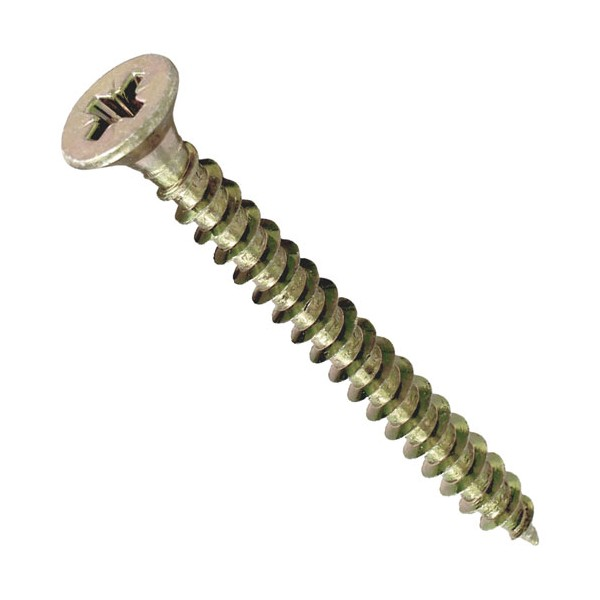
\includegraphics{screw.jpg}%
	\caption{I can't resist the temptation of showing you a screw, so here it is.}%
\end{marginfigure}%
Millions of screws come out of the production chain, and we can't test all of them.
Therefore, we need to assess the production quality by selecting at random a small set of $n$ screws, and we measure their lengths $x_1, \ldots, x_n$.
Since these lengths are highly concentrated around the theoretical desired length $\mu$, and since production errors are usually small, we decide to choose a Gaussian model: we assume that $x_i = X_i(\omega)$ for $X_i \sim \nor(\mu, \sigma^2)$, where $\sigma^2$ corresponds to a variance coming from the (hopefully) small production errors.

\emph{A model is a simplification of the reality.} For this example, we make the following modeling assumptions.
\begin{description}
	\item[Distribution choice.] We choose the distribution $\nor(\mu, \sigma^2)$ for the lengths. So, we implicitly assume that the true underlying distribution of the lengths is \emph{symmetrical} and highly \emph{concentrated} around $\mu$. This may or may not be realistic.%
	\sidenote{A real random variable $X$ is \emph{symmetrical} whenever $\P_X = \P_{-X}$. This means that $\P(X \leq -x) = \P(X \geq x)$ so that $F(-x) = 1 - F(x_-)$ if $F$ is the distribution function of $X$. Also, if $X$ has a density $f$ with respect to the Lebesgue measure, then $f$ is an even function.}
	\item[The iid assumption.] We will assume also that $X_i$ are iid. What this means in practice is that we need to very careful in the way we select the screws coming out of the production lines: for instance, we should pick screws all along a week or a month, at different times, and not all from the same production line, in order to avoid time and machine biases.
\end{description}

Once again, a statistical model is always a simplification and an approximation of the truth.
By \emph{truth} we mean the true distribution $\P_{(X_1, \ldots, X_n)}$ of $(X_1, \ldots, X_n)$.
For instance, the $\nor(0, 1)$ distribution has density $\phi(x) = e^{-x^2/2} / \sqrt{2 \pi}$ supported on $\R$. 
This means that realizations of a $\nor(0, 1)$ distribution can take any value in $\R$, while real samples are usually bounded.
However, we can prove that if $Z \sim \nor(0, 1)$, then $\Phi(x) := \P(Z \leq x)$ satisfies
\begin{marginfigure}
	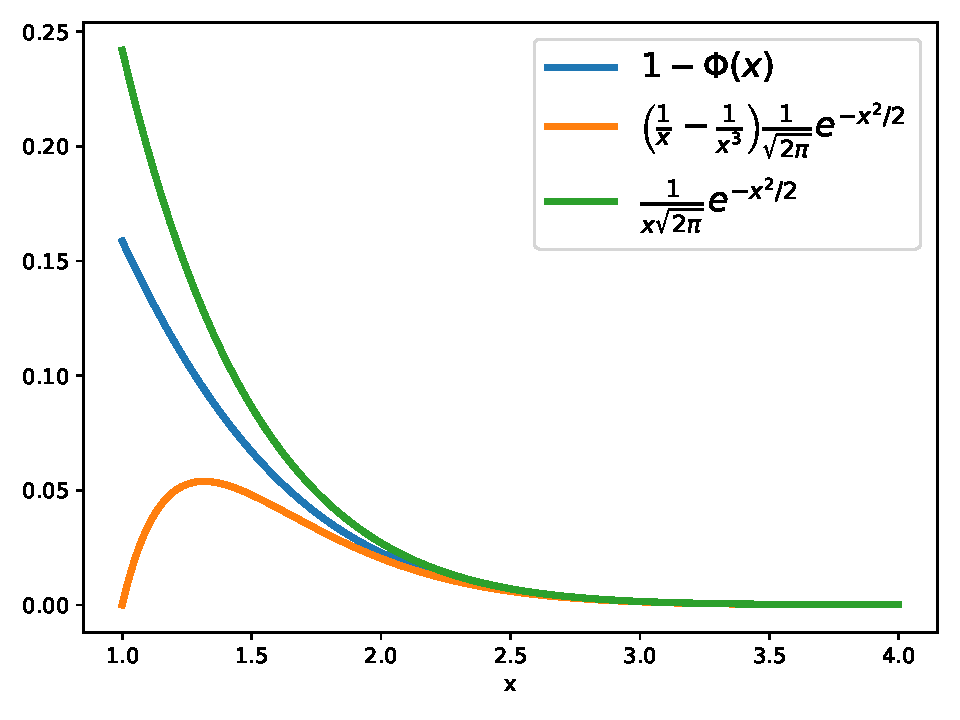
\includegraphics{images/gaussian_queue.pdf}
	\caption{Illustration of the lower and upper bounds proposed in Equation~\eqref{eq:gaussian_queue}.}
\end{marginfigure}%
\begin{equation}
	\label{eq:gaussian_queue}
	\Big( \frac 1x - \frac{1}{x^3} \Big) \frac{1}{\sqrt{2\pi}} e^{-x^2 / 2} \leq 1 - \Phi(x) \leq \frac{1}{x \sqrt{2 \pi}} e^{-x^2 / 2}
\end{equation}
for any $x > 1$, which means that the \emph{queue}%
\sidenote{The \emph{queue} of a real random variable $Z$ is the function $x \mapsto \P(Z > x)$.}%
of the $\nor$ distribution is very tight.
For $x=6$ for instance, we have $\P(Z > x) \leq 10^{-9}$: we will actually never see realizations of $\nor(0, 1)$ outside of $[-6, 6]$, and rarely outside of $[-3, 3]$.
\begin{definition}
	\label{def:statistical_experiment}
	A \emph{statistical experiment} consists of the following two things:
	\begin{itemize}
		\item A \emph{random object} $X$ valued in a probability space $(E, \cE)$
		\item A \emph{family of distributions} $\cP = \{ P_\theta : \theta \in \Theta\}$ on $(E, \cE)$.
	\end{itemize}
	We suppose that $\P_X = \P \circ X^{-1} \in \cP$. We say that $\cP$ is a \emph{statistical model} for $X$ and we will denote the statistical experiment as $(X, \cP)$.
	We call $\Theta$ the \emph{set of parameters} of the model.
\end{definition}
\marginnote{We call $X$ a \emph{random object} in Definition~\ref{def:statistical_experiment} to stress that it can be a real random variable, a random vector, a random matrix, among other things.}
The random variable $X : (\Omega, \cA, \P) \rightarrow (E, \cE)$ has distribution $\P_X = \P \circ X^{-1}$ which is the probability image of $\P$ by $X$ on $(\Omega, \cA)$.
We will always suppose that there is a family $\{ \P_\theta : \theta \in \Theta\}$ on $(\Omega, \cA)$ that induce $\{ P_\theta : \theta \in \Theta\}$ on $(E, \cE)$ and we will use the notations
\begin{equation*}
	P_\theta(A) = \P_\theta(X \in A) = \P_\theta[ \{ \omega \in \Omega : X(\omega) \in A \}] \quad \forall A \in \cE.
\end{equation*}
Let us insist on the fact that $(\Omega, \cA, \P)$ is a purely mathematical build that has no interest in statistics.
We could even assume that $X$ is the identity function and that $(\Omega, \cA) = (E, \cE)$.
Because of the transfer formula
\begin{equation*}
	\int f(X(\omega)) \P_\theta(d \omega) = \int f(x) P_\theta(dx),
\end{equation*}
we can work only with $P_\theta$ and forget about $\P_\theta$ and the space $(\Omega, \cA)$.

We will often work with a space of finite-dimensional parameters $\Theta \subset \R^d$, which corresponds to the setting  of a \emph{parametric} model, but this space can be much more complicated (it can be a set of functions with some smoothness properties for instance, such a case is covered by a field called \emph{non-parametric} statistics).
We will use the notation
\begin{equation*}
	\E_Q f(Y) := \int f(y) Q(dy)
\end{equation*}
where we implicitly assume, when computing this expectation, that $Y \sim Q$, and whenever $Q = P_\theta$, we will shorten this notation as follows:
\begin{equation*}
	\E_\theta f(X) := \E_{\P_\theta} f(X) = \int f(x) P_\theta(dx).
\end{equation*}
We will never work on $(\Omega, \cA, \P)$ but rather on $(E, \cE)$ and with the family $\cP$ (the statistical model).
\marginnote{We will quickly forget to distinguish between $\P_\theta$ and $P_\theta$ and between $\P_\theta^{\otimes n}$ and $P_\theta^{\otimes n}$. And, once again, since we are particularly lazy, we will also write $P_\theta$ instead of $P_\theta^{\otimes n}$, when there is little doubt about what we are computing.}
\begin{definition}[Sampled statistical experiment]
We have observations $X = (X_1, \ldots, X_n)$ with $X_i$ iid and $\cP = \{ P_\theta^{\otimes n} : \theta \in \Theta\}$, namely for $A = \prod_{i=1}^n A_i$ we have
\begin{align*}
	P_\theta^{\otimes n}(A) &= \P_\theta^{\otimes n}( (X_1, \ldots, X_n) \in A_1 \times \cdots \times A_n) \\
	&= \prod_{i=1}^n \P_\theta(X_i \in A_i) = \prod_{i=1}^n P_\theta(A_i).
\end{align*}
\end{definition}

\section{Statistics}
\label{sec:statistics}

Now, let us go back to the $\ber(\theta)$ experiment.
Let us first recall that for this experiment we have iid samples $X = (X_1, \ldots, X_n)$, that
$(E, \cE) = (\{0, 1\}^n, \cP(\{0, 1\}^n))$ and that $P_\theta^{\otimes n} = \ber(\theta)^{\otimes n}$ with $\Theta = (0, 1)$.
Intuitively, an ``equivalent'' experiment is $S := \sum_{i=1}^n X_i$ and $(E, \cE) = (\{ 0, \ldots, n\}, \cP(\{0, \ldots, n\}))$ with $\Theta = (0, 1)$.
Let us observe that
\begin{equation}
	\label{eq:X_cond_S}
	\begin{split}
	\P_\theta (X_1 = x_1, \ldots, X_n = x_n | S = k) &= 
	\frac{\theta^k (1 - \theta)^{n-k}}{\binom{n}{k} \theta^k (1 - \theta)^{n-k}} \\
	&= \frac{1}{\binom{n}{k}}		
	\end{split}
\end{equation}
whenever $x_i \in \{ 0, 1 \}$ for $i=1, \ldots, n$ and $k = \sum_{i=1}^n x_i$, while $\P_\theta (X_1 = x_1, \ldots, X_n = x_n | S = k) = 0$ otherwise.
This proves that the conditional distribution of $(X_1, \ldots, X_n) | S$ \emph{does not depend} on $\theta$.
If we know $S$, then we can, \emph{without knowing} $\theta$, build a ``copy'' $X' = (X_1', \ldots, X_n')$ of the original sample $X$, in the sense that $X'$ has the same distribution as $X$.
This is simply achieved, as indicated by~\eqref{eq:X_cond_S}, by choosing the positions of the $S=k$ ones (among $n$ ones and zeros) uniformly at random.
This means that $X$ does not bring more information about $\theta$ than $S$, and that that $S$ is somehow ``sufficient'' from a statistical point of view.
Such a random variable is called a \emph{sufficient statistic}.
We really need at this point to tell the reader what a \emph{statistic} is.
\marginnote{Let us recall the Doob lemma. Let $X$ and $Y$ be two random variables on the same probability space. Then $Y$ is $X$-measurable (namely measurable with respect to the $\sigma$-field $\sigma(X)$ generated by $X$) if and only if there exists a measurable function $f$ such that $Y = f(X)$.}
\begin{definition}
	Given a statistical experiment $(X, \{ P_\theta : \theta \in \Theta \})$, we call \emph{statistic} any $X$-measurable function that does not depend on~$\theta$.
	A statistic is therefore a quantity that we can compute using data only.
\end{definition}
For the $\ber(\theta)$ experiment, we will look for statistics of $X$ allowing to infer the unknown parameter $\theta$.
We already now that we can restrict ourselves to statistics of $S$ instead of $X$, since $S$ is  sufficient.

\section{Identifiable models} % (fold)

The only source of information about $\theta$ available to us about is $X$, through its distribution $P_{\theta}$.
So, in order to infer $\theta$, we need, at least, to be able to recover $\theta$ given $P_\theta$.
We will therefore often require that the model is \emph{identifiable}, as defined below.
\begin{definition}
	We say that a model $\cP = \{ P_\theta : \theta \in \Theta \}$ is \emph{identifiable} whenever the function $\Theta \rightarrow \cP$ given by $\theta \mapsto P_\theta$
	is \emph{injective}.
\end{definition}
Identifiability is a necessary requirement when one wants to perform statistical inference.
If $\theta \mapsto P_\theta$ is not injective, then there is no way to find back $\theta$ from $X \sim P_\theta$.

\begin{example}
	\label{ex:identifiabiliy}
	Obviously, $\theta \mapsto \ber(\theta)$ is injective on $(0, 1)$ and similarly $x \mapsto \ber(\sigmoid(x))$ is injective on $\R$.
	A stupid example is $\mu \mapsto \nor(\mu^2, 1)$ on $\R$, which corresponds to a non-identifiable model.
\end{example}
In Example~\ref{ex:identifiabiliy}, we used the sigmoid function given by $\sigmoid(x) = 1 / (1 + e^{-x})$ for any $x \in \R$.%
\sidenote{The sigmoid function is heavily used in statistics and machine learning, we will come back to it later in the book.}
Identifiability is generally a property that we ensure by choosing and parametrizing correctly the considered statistical model.
An interesting example of \emph{non-identifiable} model is given by \emph{mixture models}, such as the Gaussian mixture model, where we consider a distribution on $\R^d$ with density
\sidenote{In the paramatrization of the Gaussian mixture we have expectations $\mu_k \in \R^d$ that correspond to the centroids of the clusters, we have covariances $\bSigma_k \in \R^{d \times d}$ such that $\bSigma_k \succ 0$, which means that $\bSigma_k$ is a symmetric and positive matrix, that parametrizes the shape cluster $k$ around its centroid and finally we have $\pi_k \geq 0$ that are such that $\sum_{k=1}^K \pi_k = 1$ and parametrize the relative population of each cluster.}%
\begin{align*}
	f_\theta(x) &= \sum_{k=1}^K \pi_k \phi_{\mu_k, \bSigma_k}(x) \\ 
	&=: \sum_{k=1}^K \frac{\pi_k }{\sqrt{(2 \pi)^d \det (\bSigma_k)}} 
	\exp\Big( -\frac 12 (x - \mu_k)^\top \bSigma_k^{-1} (x - \mu_k) \Big)
\end{align*}
\begin{marginfigure}
	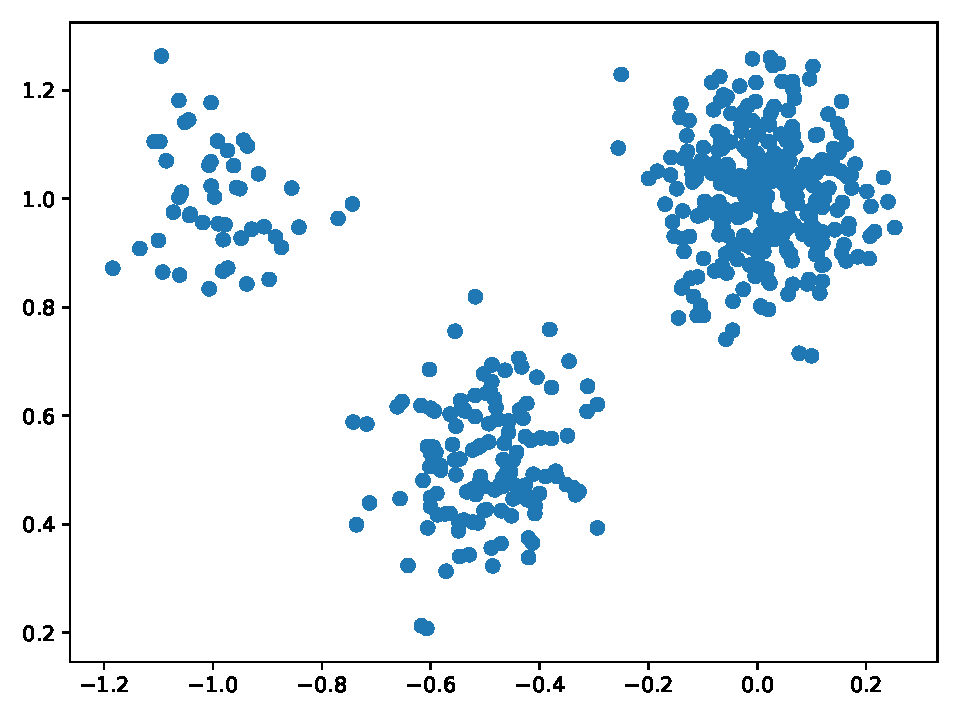
\includegraphics{images/gmm.pdf}
	\caption{$500$ realizations of a Gaussian mixture with $d=2$, $K=3$ and the following parameters $\pi = [\pi_1, \pi_2, \pi_3] = [0.1, 0.6, 0.3]$, $\mu_1 = [-1, 1]$, $\mu_2 = [0, 1]$, $\mu_3 = [-0.5, 0.5]$ and $\bSigma_1 = \bSigma_2 = \bSigma_3 = 0.01 \times \bI_2$.}
\end{marginfigure}
for any $x \in \R^d$, where $\theta = (\pi_k, \mu_k, \bSigma_k)_{k=1, \ldots, K}$ and $K \geq 1$ is an integer corresponding to the number of ``clusters''.
Such a mixture density is non-identifiable, since we have $f_{\theta} = f_{\sigma(\theta)}$
for any permutation $\sigma(\theta) = (\pi_{\sigma(k)}, \mu_{\sigma(k)}, \bSigma_{\sigma(k)})_{k=1, \ldots, K}$ of $\theta$ where $\sigma$ is a permutation of $\{1, \ldots, K \}$.
This simply means that the density distribution $f_\theta$ is invariant by a relabeling of the clusters numbers.
Despite the fact that such a mixture model is not identifiable, it is often used for \emph{model-based clustering}, which is an instance of \emph{unsupervised learning}.
Another family of non-identifiable models is deep neural networks, in which an infinitely large number of parametrizations lead to the same prediction function.

\section{Dominated models} 

Whenever $\cP = \{ P_\theta : \theta \in \Theta \}$ with $\Theta \subset \R^d$, we say that $\cP$ is a \emph{parametric} model, since it is parametrized by a finite-dimensional parameter, trivial instances being $\{ \ber(\theta) : \theta \in (0, 1) \}$ for which $d=1$ and $\{ \nor(\mu, v) : (\mu, v) \in \R \times (0, +\infty) \}$ for which $d=2$.
We say that both models are \emph{dominated}, the first being dominated by the counting measure $\nu = \delta_0 + \delta_1$ on $\{ 0, 1\}$,%
\sidenote{The notation $\delta_x$ will stand for the Dirac mass at $x$ which is the probability measure satisfying $\int f(u) \delta_x(du) = f(x)$ for any measurable function $f$.}%
and the second by the Lebesgue measure on $\R$.\sidenote{We recall that if $P$ and $Q$ are two measures on the same probability space, $P \ll Q$ means that the measure $P$ is \emph{absolutely continuous} with respect to $Q$, namely that $Q(A) = 0 \Rightarrow P(A)= 0$ for any measurable set $A$.}
\begin{definition}
	\label{def:dominated-model}
	We say that a model $\cP = \{ P_\theta : \theta \in \Theta \}$ is dominated if there is a $\sigma$-finite measure $\mu$ such that $P_\theta \ll \mu$ for all $\theta \in \Theta$.
\end{definition}
In Definition~\ref{def:dominated-model}, we require that the dominating measure is $\sigma$-finite, so that we can apply the Radon-Nikodym theorem: since $P_\theta \ll \mu$ for all $\theta \in \Theta$, there is a density 
\begin{equation*}
	f_\theta = \frac{dP_\theta}{d\mu}
\end{equation*}
for all $\theta \in \Theta$.
This domination property allows to work with densities instead of distributions: a model can be therefore defined as a family of densities $\{ f_\theta : \theta \in \Theta \}$ together with a dominating measure (which is in most cases the Lebesgue measure, a counting measure, or a combination of them.)
\begin{example}
	Let us consider the \emph{zero-inflated Laplace distribution}, which is a distribution on $\R$ given by
	\begin{equation*}
		P_\theta(dx) = \pi_0 \delta_0(dx) + (1 - \pi_0) \frac{\lambda}{2} e^{-\lambda |x|} dx
	\end{equation*}
	for $\theta = (\pi_0, \lambda) \in \Theta = (0, 1) \times (0, +\infty)$, which is dominated by the measure $\mu = \delta_0 + \leb$, where $\leb$ stands from now on for the Lebesgue measure on $\R$.
\end{example}
Non-dominated models are usually pathological and uninteresting examples, such as the model
\begin{equation*}
	P_\lambda = \frac 1e \sum_{n \geq 0} \frac{1}{n!} \delta_{\lambda n}
\end{equation*}
for $\lambda \in (0, +\infty)$, which cannot be dominated by a $\sigma$-finite measure.

Let us finish this chapter with an example of non-parametric model: we observe $X_1, \ldots, X_n$ with a density $f \in F$ with respect to the Lebesgue measure, where $F$ is the set of probability densities on $[0, 1]^d$ that are $C^2$ and such that $\grad^2 f(x) \mleq L \bI_d$.%
\sidenote{The notation $\nabla^2 f(x)$ stands for the Hessian matrix of $f$, while $\bI_d$ is the identity matrix on $\R^d$. Finally, for two symmetric matrices $\bA$ and $\bB$, the notation $\bA \mleq \bB$ means $\bB - \bA \mgeq 0$, namely that $\bB - \bA$ is a symmetric and positive semi-definite matrix.}%
In such a setting, we work with an infinite dimensional set of parameters $F$, and need to build a \emph{non-parametric} estimator of the unknown density $f$.



\setchapterpreamble[u]{\margintoc}
\chapter{Statistical inference}
\label{chap:statistical_inference}

In this Chapter, we will consider all along the simple Bernoulli model, where we have iid samples $X_1, \ldots, X_n$ distributed as $\ber(\theta)$ with $\theta \in (0, 1)$.
Let us start with the first \emph{inference} problem: the \emph{estimation} problem.

\section{Estimation} % (fold)
\label{sec:estimation}

We want to \emph{infer} $\theta$, or \emph{estimate} it by finding a statistic which is a measurable function of $(X_1, \ldots, X_n)$%
\sidenote{Once again, since we are doing statistics, the only thing we are allowed to use is the data.}%
or a measurable function of $S_n = \sum_{i=1}^n X_i$ thereof, since $S_n$ is sufficient, see Section~\ref{sec:statistics}.
We will denote such a statistic as
\begin{equation*}
 	\wh \theta_n = \wh \theta(X_1, \ldots, X_n).
\end{equation*}
This function \emph{does not depend} on $\theta$, but its distribution does.
Ideally, we want $\wh \theta_n$ to be ``close'' to $\theta$, since we want a good estimator, so that the first thing we need to do is to quantify ``closeness''.
For instance, we could want $|\wh \theta_n - \theta|$ to be close to $0$ with a large probability, since we do not forget that $\wh \theta_n$ is a random variable, as a function of the data $(X_1, \ldots, X_n)$.
The most natural distance is arguably the Euclidean one, in this context the $L^2$ distance, 
which leads to the \emph{quadratic risk}.%
\sidenote{Although the quadratic risk corresponds to a \emph{squared} $L^2$ norm.}
\begin{definition}[Quadratic risk]
	\label{def:quadratic_risk}
	Consider a statistical model with data $X$ and set of parameters $\Theta \subset \R$ and an estimator $\wh \theta(X)$. 
	The quadratic risk of $\wh \theta$ is given by
	\begin{equation*}
		R(\wh \theta, \theta) = \E_\theta[ (\wh \theta - \theta)^2 ] = \int_E (\wh \theta(x) - \theta)^2 P_\theta(dx).
	\end{equation*}
	We consider the quadratic risk as a function $\Theta \goes \R^+$ of the parameter given by $\theta \mapsto R(\wh \theta, \theta)$.
\end{definition}
At this point, it's useful to recall some classical inequalities on the queues of random variables.
The Markov inequality tells us that if $Y$ is a real random variable such that $\E |Y|^p < +\infty$ for some $p > 0$ then
\begin{equation*}
	\P(|Y| > t) \leq \frac{\E |Y|^p}{t^p}
\end{equation*}
for any $t > 0$.
This tells us that the more $Y$ has moments%
\sidenote{We say that $Y$ as moments up to order $p$ if $\E |Y|^p < +\infty$. 
Note that this entails $\E |Y|^q < +\infty$ for any $q < p$ since $\E |Y|^p = \E (|Y|^q)^{p/q} \geq (\E |Y|^q)^{p/q}$ using Jensen's inequality.}%
the more the queue of $Y$ is tight (it goes faster to $0$ with $t \goes +\infty$).
Markov's inequality with $p=2$ entails 
\begin{equation}
	\label{eq:l2_entrails_proba}
	\P(|\wh \theta - \theta| > t) \leq \frac{R(\wh \theta, \theta)}{t^2}
\end{equation}
which tells us that whenever the quadratic risk is small, then $\wh \theta$ is close to $\theta$ with a large probability.

Whenever $R(\wh \theta_n, \theta) \rightarrow 0$ with $n \rightarrow +\infty$, we will write $\wh \theta_n \goqr \theta$, which stands for convergence in $L^2$ norm, which entails, because of Inequality~\eqref{eq:l2_entrails_proba}, that $\wh \theta_n \gopro \theta$, which stands for convergence in probability.\sidenote{More precisely, in $\P_\theta$-probability, namely $\P_\theta[|\wh \theta_n - \theta| > \eps] \rightarrow 0$ as $n \rightarrow +\infty$ for any $\eps > 0$, but we will write $\wh \theta_n \gopro \theta$ in order to keep the notations as simple as possible.}%
\begin{definition}
	\label{def:consistent}
	We say that $\wh \theta_n$ is \emph{consistent} whenever $\P_\theta[|\wh \theta_n - \theta| > \eps] \rightarrow 0$ as $n \rightarrow +\infty$ for any $\eps > 0$ and any $\theta \in \Theta$.
	We say that it is strongly consistent whenever $\P_\theta[\wh \theta_n \rightarrow \theta] = 1$ for any $\theta \in \Theta$.
\end{definition}
In Definitions~\ref{def:quadratic_risk} and~\ref{def:consistent} above, if $\Theta \subset \R^d$, it suffices to replace $|\cdot|$ by the Euclidean norm $\norm{\cdot}_2$.%
\sidenote{We can use any norm on $\R^d$ in Definition~\ref{def:consistent}, and let us recall that $\norm{x}_2 = \sqrt{x^\top x} = (\sum_{j=1}^d x_j^2)^{1/2}$.}%

\paragraph{Bias variance decomposition.} % (fold)

The \emph{bias-variance decomposition} is the following decomposition of the quadratic risk between two terms: a bias term denoted $b(\wh \theta_n, \theta)$ (squared in the formula) and a variance term:
\begin{equation}
	\label{eq:bias-variance-decomposition}
	\begin{split}
	R(\wh \theta_n, \theta) &= \E_\theta[(\wh \theta_n - \theta)^2] = (\E_\theta \wh \theta_n - \theta)^2 + \var_\theta(\wh \theta_n) \\
	&= b(\wh \theta_n, \theta)^2 + \var_\theta(\wh \theta_n).		
	\end{split}
\end{equation}
When $b(\wh \theta_n, \theta) = 0$ for all $\theta \in \Theta$ we say that the estimator $\wh \theta_n$ is \emph{unbiased}.
This means that this estimator will not tend to over or under-estimate $\theta$. 

\paragraph{Back to Bernoulli.} % (fold)

% paragraph back_to_bernoulli (end)Back to Bernoulli
Going back to the $\ber(\theta)$ model, we consider the estimator $\wh \theta_n = S / n = \sum_{i=1}^n X_i / n$.
We already know many things about this estimator:
\begin{enumerate}
	\item We have $\E_\theta [\wh \theta_n] = \theta$ which means that $\wh \theta_n$ is unbiased;
	\item The bias-variance decomposition gives
	\begin{equation}
		\label{eq:bernoulli-quadratic-risk}
	 	R(\wh \theta_n, \theta) = \var(\wh \theta_n) = \frac{\theta (1 - \theta)}{n} \leq 
	 	\frac{1}{4 n} \rightarrow 0
	 \end{equation}
	 which means that $\wh \theta_n \goqr \theta$ and which entails that $\wh \theta_n$ it is consistent;
	\item The law of large number tells us that $\wh \theta_n \goas \theta$, hence $\wh \theta_n$ is strongly consistent;
	\item The central limit theorem tells us that
	\begin{equation}
	\label{eq:tcl-bernoulli}
	\sqrt n (\wh \theta_n - \theta) \leadsto \nor(0, \theta(1 - \theta)).
	\end{equation}
\end{enumerate}
The points 2--4 from above are all different ways of saying that when $n$ is large enough, then $\wh \theta_n$ is close to $\theta$.
In practice, an estimator leads to a value: for the Bernoulli model with $n=100$ and $42$ ones you end up with a single estimated value $0.42$.
But what if we want to include uncertainty in this estimation ?
Namely how confident are we about this $0.42$ value ?
Moreover, what do we mean by ``when $n$ large enough'', can we quantify this better ?
All these questions can be answered by considering another inference problem: confidence intervals.

\section{Confidence intervals} % (fold)
\label{sec:confidence_intervals}

Here, we don't only want to build an estimator $\wh \theta_n$ but also to quantify the uncertainty of this estimation.
Combining Inequalities~\eqref{eq:l2_entrails_proba} and~\eqref{eq:bernoulli-quadratic-risk} leads to
\begin{equation*}
	\P_\theta[ |\wh \theta_n - \theta| > t] \leq \frac{1}{4 n t^2}
\end{equation*}
so that for $\alpha \in (0, 1)$ and the choice $t_\alpha = 1 / (2 \sqrt{n \alpha})$ we have 
\begin{equation*}
	\P_\theta \{ \theta \in [ \wh \theta^L, \wh \theta^R ] \} \geq 1 - \alpha,
\end{equation*}
where
\begin{equation*}
	\wh \theta^L =  \wh \theta_n - \frac{1}{2 \sqrt{n \alpha}} \quad \text{ and } \quad \wh \theta^R =  \wh \theta_n + \frac{1}{2 \sqrt{n \alpha}}.
\end{equation*}
Therefore, if we choose $\alpha = 0.05 = 5\%$, we know that $\theta \in [\wh \theta^L, \wh \theta^R]$ with a probability larger than $95\%$.
We say in this case that the interval $[\wh \theta^L, \wh \theta^R]$ is a \emph{confidence interval} with coverage $95\%$.%
\sidenote{If we toss the coin $1000$ times and get $420$ heads, the realization of this confidence interval at $95\%$ is $[0.35, 0.49]$.}

Note that if $\alpha = 0$ then we have no other choice than using the whole $\R$ as a confidence interval: $\alpha$ allows to give some slack, so that we can build a non-absurdly  large confidence interval. 
We typically have that $|\wh \theta^R - \wh \theta^L|$ increases as $\alpha$ decreases, since a smaller $\alpha$ means more confidence, hence a larger interval.
On the contrary, $|\wh \theta^R - \wh \theta^L|$ should decrease with the sample size $n$.
\begin{definition}[Confidence interval]
	Consider a statistical model with data $X$ and set of parameters $\Theta \subset \R$. 
	Fix a \emph{confidence level} $\alpha \in (0, 1)$ and consider two statistics $\wh \theta^L(X)$ and $\wh \theta^R(X)$. Whenever 
	\begin{equation}
		\label{eq:coverage-property}
		\P_\theta\{ \theta \in [\wh \theta^L(X), \wh \theta^R(X)] \} \geq 1 - \alpha
	\end{equation}
	for any $\theta \in \Theta$, we say that $[\wh \theta^L(X), \wh \theta^R(X)]$ is a \emph{confidence interval} at level $1 - \alpha$.
\end{definition}
Inequality~\eqref{eq:coverage-property} is called the \emph{coverage} property of the confidence interval.
More generally, when $\Theta \subset \R^d$, we will say that $S(X)$ is a \emph{confidence set} if it is a statistic satisfying the coverage property $\P_\theta\{ \theta \in S(X) \} \geq 1 - \alpha$ for any $\theta \in \Theta$.
\begin{remark}
	Whenever we need only an upper or lower bound on $\theta$ (for instance, when we need to check statistically that some toxicity level is below some threshold), we build a \emph{unilateral} or \emph{one-sided} confidence interval, where we choose either $\wh \theta^L = -\infty$ ($0$ for the Bernoulli model) or $\wh \theta^R = +\infty$ ($1$ for the Bernoulli model).
	Indeed, at a fixed level $1 - \alpha$, the bound of a one-sided confidence interval is tighter than the same sided bound corresponding to a two-sided interval. 
\end{remark}
But, we can do better for the Bernoulli model (or any model where $X$ is bounded) thanks to the following Hoeffding inequality.
\begin{theorem}
	\label{thm:hoeffding}
	Let $X_1, \ldots, X_n$ be independent random variables such that $X_i \in [a_i, b_i]$ almost surely and let $S = \sum_{i=1}^n X_i$. Then,
	\begin{equation*}
		\P[ S \geq \E S + t] \leq \exp\Big( - \frac{2 t^2}{\sum_{i=1}^n (b_i - a_i)^2} \Big)
	\end{equation*}
	holds for any $t >0$.
\end{theorem}
Theorem~\ref{thm:hoeffding} is something called a deviation inequality: it provides a control on the probability of deviation of $S$ with respect to its mean.
It shows that bounded random variables are \emph{sub-Gaussian}, since it shows that the queue of $S - \E S$ is bounded by $\exp(-c t^2)$ for some constant $c$ (that depends on $n$).
The proof of this inequality is provided in Chapter~??\todo{insert reference} below.
\todo{Provide the proof of Hoeffding}

\paragraph{Back to Bernoulli.} % (fold)

% paragraph back_to_bernoulli (end)
Let's apply Theorem~\ref{thm:hoeffding} to the Bernoulli model $X_i \sim \ber(\theta)$ so that $a_i = 0$, $b_i = 1$ and therefore $\P[ S \geq \E S + t] \leq e^{-2 t^2 / n}$.
Using again Theorem~\ref{thm:hoeffding} with $X_i$ replaced by $-X_i$ together with an union bound%
\sidenote{}%
leads to $\P[ | S - \E S | \geq t] \leq 2 e^{-2 t^2 / n}$.
So, for some $\alpha \in (0, 1)$, we obtain another confidence interval, since the following coverage property holds:
\begin{equation*}
	\P \bigg[ \wh \theta_n - \sqrt{\frac{\log(2 / \alpha)}{2n}} \leq \theta \leq \wh \theta_n 
	+ \sqrt{\frac{\log(2 / \alpha)}{2n}} \bigg] \geq 1 - \alpha.
\end{equation*}
This proves that $[\wh \theta \pm \sqrt{\log(2 / \alpha) / (2n)}]$ is a confidence interval at level $1 - \alpha$.%
\sidenote{For $1000$ tosses and $420$ heads, the realization of this interval at level $95\%$ is $[0.37, 0.46]$. It's a bit more precise than the previous one, which was based on Markov's inequality.}
Let's compare the two confidence intervals we obtained so far for the Bernoulli model.
We have of course
\begin{equation*}
	\frac{1}{2 \sqrt{n \alpha}} > \sqrt{\frac{\log(2 / \alpha)}{2n}} 
\end{equation*}
for $\alpha$ small enough\todo{etre plus precis ici}, although both sides are $O(1 / \sqrt n)$.
Only the dependence on the level $\alpha$ is improved with the confidence interval obtained through Hoeffding's inequality, since it exploits the sub-Gaussianity of the Bernoulli distribution, while the first confidence interval only used the upper bound~\eqref{eq:l2_entrails_proba} on the variance.%
\sidenote{There is yet another way to build a (non-asymptotic) confidence interval, using a more computational approach, see for instance ????}

\paragraph{Asymptotic coverage.}

For both the previous confidence intervals, we adopted a \emph{non-asymtotic} approach: the coverage properties hold for any value of $n \geq 1$.
This is possible since we know things about the distribution of $S$, which is a simple $\bin(n, \theta)$ distribution.
However, in general, the \emph{exact} distribution of an estimator $\wh \theta_n$ cannot always be made explicit, and in such cases, we often use Gaussian approximations, thanks to the central limit theorem. 
Let's do this for the Bernoulli model.
Indeed, we know from~\eqref{eq:tcl-bernoulli} that
\begin{equation}
	\label{eq:portemanteau-bernoulli}
	\P_\theta \bigg[ \sqrt{\frac{n}{\theta (1 - \theta)}} (\wh \theta_n - \theta) \in I
	\bigg] \rightarrow \P[Z \in I]
\end{equation}
where $Z \sim \nor(0, 1)$ for any closed interval $I \subset \R$.%
\sidenote{This uses the porte-manteau theorem, which says that $X_n \gosto X$ if and only if $\P(X_n \in A) \goes \P(X \in A)$ for any Borelian set $A$ such that $\P(X \in \partial A) = 0$, where $\partial A$ stands for the boundary of $A$.}%
Using $I = [-q_\alpha, q_\alpha]$ with $q_\alpha = \Phi^{-1}(1 - \alpha / 2)$ we end up%
\sidenote{We recall that $\Phi^{-1}$ is the inverse of the distribution function $\Phi(x) = \P( Z \leq x)$ of the $\nor(0, 1)$ distribution, that we call the \emph{quantile} function of $\nor(0, 1)$.}%
with the fact that
\begin{equation}
	\label{eq:not-and-ic}
	\P_\theta\bigg\{ \theta \in \Big[ \wh \theta_n \pm q_\alpha \sqrt{\frac{\theta(1 - \theta)}{n}} \Big] \bigg\} \rightarrow 1 - \alpha.
\end{equation}
This is interesting, but not enough to build a confidence interval, since the interval in Equation~\eqref{eq:not-and-ic} depends on $\theta$ through the variance term $\theta(1 - \theta)$.
Indeed, a confidence interval must be something that does \emph{not} depend on $\theta$.
We need to work a little bit more in order to remove the dependence on $\theta$ from this interval. 
We do the same as before: we use the fact that $\theta (1 - \theta) \leq 1 / 4$ for any $\theta \in [0, 1]$, so that
\begin{equation*}
	\liminf_n \P_\theta \bigg\{ \theta \in \Big [\wh \theta_n \pm \frac{q_\alpha}{2 \sqrt n} \Big] \bigg\} \geq 1 - \alpha.
\end{equation*}
This is what we call a confidence interval \emph{asymptotically of level} $1 - \alpha$ constructed \emph{by excess}.

In the above construction of an asymptotic confidence interval, we used the central limit theorem to approximate the $\bin(n, \theta)$ distribution (the distribution of $S = \sum_{i=1}^n X_i$) by a Gaussian distribution.
This requires $n$ to be ``large enough'', but the central limit theorem does not tell us how large.
We can quantify this better by trying to quantify how close the distribution function of $S$ is to the one of $\nor(0, 1)$, using the following theorem.
\begin{theorem}[Berry-Esseen]
	Let $X_1, \ldots, X_n$ be i.i.d random variables such that $\E X_i = 0$ and $\var(X_i) = \sigma^2$ and introduce the distribution function%
	\marginnote{BLABLABLA}%
	\begin{equation*}
		F_n(x) = \P \bigg[ \frac{\sum_{i=1}^n X_i}{\sqrt{n \sigma^2}} \leq x \bigg]
	\end{equation*}
	for any $x \in \R$. Then, the following inequality holds:
	\begin{equation*}
		\sup_{x \in \R} |F_n(x) - \Phi(x)| \leq \frac{c \kappa}{\sigma^3 \sqrt n},
	\end{equation*}
	where $\kappa = \E |X_1|^3$ (assumed finite) and where $c$ is a purely numerical constant (the best known one is $c = 0.4748$).
\end{theorem}
We provide a proof with a worse constant $c$ in Section~??? below.\todo{insert proof}
Note that there is also a lower bound with $c \geq 0.4097$, as explained in ?? and that the best constant $c = 0.4748$ for the upper bound is from ???.
Note also that a similar result holds if the $X_i$ are independent but not identically distributed.

For Bernoulli with have $\E|X_1|^3 = \theta$ and $\sigma^3 = (\theta(1 - \theta))^{3/2}$ so that 
\begin{equation*}
	|F_n(x) - \Phi(x)| \leq \frac{3}{\sqrt{n \theta (1 - \theta)^3}}
\end{equation*}
which shows that the approximation by the Gaussian distribution deteriorates whenever $\theta$ is close to $0$ or $1$.

\paragraph{Reparametrization.} % (fold)

Another asymptotic approach allowing to get rid of the dependence on $\theta$ in the confidence interval~\eqref{eq:not-and-ic} is based on the idea of reparametrization.
Indeed, given a statistical model $\{ P_\theta : \theta \in \Theta \}$ and a bijective function $g : \Theta \goes \Lambda$ we can use instead the ``reparametrized''model $\{ Q_\lambda : \lambda \in \Lambda \}$ where $Q_\lambda = P_{g^{-1}(\lambda)}$.
Let us also remark that if $[\wh \theta^L, \wh \theta^R]$ is a confidence interval for $\theta$ at level $1 - \alpha$ and if $g$ is an increasing function, then 
$[g(\wh \theta^L), g(\wh \theta^R]$ is a confidence interval for $g(\theta)$ at level $1 - \alpha$.
Now, a natural question is to understand if the convergences we used above (in particular, the convergence in distribution involved in the central limit theorem) is stable under such a reparametrization.
\begin{example}
	\label{ex:expo}
	Consider a iid dataset $X_1, \ldots, X_n$ with distribution $\expo(\theta)$ with scale parameter $\theta > 0$, namely the distribution $P_\theta(dx) = \theta e^{-\theta x} \ind{x \geq 0} dx$. 
	We have $\E(X_1) = 1 / \theta$ and $\var(X_1) = 1 / \theta^2$, so that using the law of large numbers and the central limit theorem we have
	\begin{equation*}
		\bar X_n \goas \theta^{-1} \quad \text{ and } \quad \sqrt n (\bar X_n - \theta^{-1}) \leadsto \nor(0, \theta^{-2})
	\end{equation*}
	when $n \rightarrow +\infty$.
	Since $x \mapsto 1 / x$ is a continuous function on $(0, +\infty)$, we know that $(\bar X_n)^{-1} \goas \theta$ so that a strongly consistent estimator is given by $\wh \theta = (\bar X_n)^{-1}$.
	But what can we say about the convergence in distribution of 
	$\sqrt n (\wh \theta_n - \theta)$ ?
\end{example}
This is answered by so-called $\Delta$-method, described in the next theorem.
\begin{theorem}[$\Delta$-method]
	\label{thm:delta-method}
 	Let $(Z_n)_{n \geq 1}$ be a sequence of real random variables and assume that 
	$a_n(Z_n - z) \leadsto Z$, where $(a_n)_{n \geq 1}$ is a positive sequence such that $a_n \goes +\infty$, where $z \in \R$ and where $Z$ is a real random variable.
 	If $g$ is a function defined on a neighborhood of $z$ and differentiable at $z$, we have 
 	\begin{equation}
 		a_n (g(Z_n) - g(z)) \leadsto g'(z) Z
 	\end{equation}
 	as $n \goes +\infty$.
\end{theorem}
The proof easily follows from a first-order Taylor expansion of $g$ around~$z$, as explained in Section~??? below. \todo{insert proof}
A particularly useful case for statistics is when $Z$ is Gaussian.
For instance, if $\sqrt n (\wh \theta_n - \theta) \leadsto \nor(0, \sigma(\theta)^2)$, we have
\begin{equation*}
	\sqrt n (g(\wh \theta_n) - g(\theta)) \leadsto 
	\nor(0, \sigma(\theta)^2 (g'(\theta))^2)
\end{equation*}
whenever $g$ satisfies the conditions of Theorem~\ref{thm:delta-method}.
Going back to the $\expo(\theta)$ example from Example~\ref{ex:expo}, we obtain with $g(x) = 1 / x$ and since $\wh \theta = g(\bar X_n)$ that $\sqrt n (\wh \theta - \theta) \leadsto \nor(0, \theta^2)$.
Another result which provides stability for the convergence in distribution under a smooth mapping is the so-called Slutsky theorem.
\begin{theorem}[Slutsky]
	\label{thm:slutsky}
	Let $(X_n)_{n \geq 1}$ and $(Y_n)_{n \geq 1}$ be sequences of real random variables such that $X_n \leadsto X$ and $Y_n \leadsto y$ where $X$ is some real random variable and $y \in \R$.
	Then, we have that $Y_n \gopro y$ and $(X_n, Y_n) \leadsto (X, y)$ as $n \goes +\infty$. In particular, we have $f(X_n, Y_n) \leadsto f(X, y)$ for any continuous function $f$.
\end{theorem}
The proof of Theorem~\ref{thm:slutsky} is given in Section~? below.\todo{insert proof}
The $\Delta$-method provides stability for the convergence in distribution when a differentiable function is applied to a sequence, while Slutsky theorem provides ``algebraic'' stability when combining two sequences converging respectively in distribution and probability.
\sidenote{Be careful with convergence in distribution. Please keep in mind that this mode of convergence is about the convergence of the distributions and not the convergence of the random variables (hence its name). The notation $X_n \gosto X$ is rather misleading but convenient. In particular, nothing can be said in general about $f(X_n, Y_n)$ when we know that $X_n \gosto X$ and $Y_n \gosto Y$ (unless $X_n$ and $X_n$ are independent sequences).}

\paragraph{Back again to Bernoulli.}

We have $\wh \theta_n \gopro \theta$, so that $(\wh \theta_n (1 - \wh \theta_n)^{1/2} \gopro (\theta (1 -  \theta))^{1/2}$ since $x \mapsto (x(1-x))^{1/2}$ is continuous on $[0, 1]$ and let us write
\begin{equation*}
	\frac{\sqrt n (\wh \theta_n - \theta)}{\sqrt{\wh \theta_n (1 - \wh \theta_n)}} 
	= \frac{\sqrt n (\wh \theta_n - \theta)}{\sqrt{ \theta (1 -  \theta)}} \times 
	\sqrt{\frac{ \theta (1 -  \theta)}{\wh \theta_n (1 - \wh \theta_n)}} =: A_n \times B_n.
\end{equation*}
We know that $A_n \gosto \nor(0, 1)$ and that $B_n \gopro 1$.
Therefore, using Theorem~\ref{thm:slutsky} leads%
\sidenote{With $f(x, y) = xy$.}%
to
\begin{equation*}
	\sqrt{\frac{n}{\wh \theta_n (1 - \wh \theta_n)}} (\wh \theta_n - \theta) \gosto \nor(0, 1).
\end{equation*}
Yes, we just replaced $\theta$ by $\wh \theta_n$ in the variance term $\theta(1 - \theta)$ of the limit~\eqref{eq:portemanteau-bernoulli}, but doing so required Slutsky's theorem to prove this rigorously, and this provides us another confidence interval with asymptotic coverage given by
\begin{equation*}
	\P_\theta \bigg\{ \theta \in \Big[ \wh \theta_n \pm q_\alpha \sqrt{\frac{\wh \theta_n (1 - \wh \theta_n)}{n}} \Big] \bigg\} \goes 1 - \alpha
\end{equation*}
as $n \goes +\infty$.%
\sidenote{With $1000$ tosses and $420$ heads, the realization of this confidence interval at level $95\%$ is $[0.38, 0.45]$.}%


\section{Tests} % (fold)
\label{sec:tests}

Let us consider, again, in this section, a statistical experiment with data $X$ and model $\{ P_\theta : \theta \in \Theta \}$.
Here, we want to decide between to hypothesis $H_0$ and $H_1$, where
\begin{equation*}
	H_i \quad \text{means that} \quad \theta \in \Theta_i
\end{equation*}
for $i \in \{ 0, 1 \}$, where $\{ \Theta_0, \Theta_1 \}$ is a partition of the set of parameters~$\Theta$.
In order to understand the concept of statistical testing, let us consider the following unsettling example: imagine that you need to decide if a patient has cancer or not.
The patient has cancer if some parameter $\theta \in (0, 1)$ about him satisfies
$\theta \geq 0.42$.
We \emph{choose} $\Theta_0 = [0.42, 1]$ and $\Theta_1 = [0, 0.42)$, namely we decide that $H_0$ means that the patient has cancer, while $H_1$ means that the patient has not.
We need to construct a testing function $\varphi : E \goes \{ 0, 1 \}$ that maps $X \mapsto \varphi(X)$, our decision being given by the value of $\varphi(X)$. 
We decide that $H_0$ is true whenever $\varphi(X) = 0$, in this case we say that we \emph{accept} $H_0$ and we \emph{reject} $H_0$ whenever $\varphi(X) = 1$.
This is a convention, the $1$ in $\varphi(X) = 1$ and $H_1$ will always mean that we \emph{reject} the \emph{null hypothesis} $H_0$.

\paragraph{Type I and Type II errors.}

When $\theta \in \Theta_i$, we are correct if $\varphi(X) = i$ and incorrect if $\varphi(X) = 1 - i$.
We have two types of errors: the \emph{Type-I error}, also called the \emph{first-order error}, given by 
\begin{equation}
	\label{eq:type-1-error}
	\P_\theta[ \varphi(X) = 1] = \E_\theta [\varphi(X)] \quad \text{for} \quad
	\theta \in \Theta_0
\end{equation}
and the \emph{Type-II error}, also called \emph{second-order error}, given by 
\begin{equation}
	\label{eq:type-2-error}
	\P_\theta[ \varphi(X) = 0] = 1 - \E_\theta [\varphi(X)] \quad \text{for} \quad 
	\theta \in \Theta_1.
\end{equation}
For the cancer detection problem, the Type~I error corresponds to the \emph{probability of saying to the patient that he has not cancer while he has.}
The Type~II error corresponds to the \emph{probability of saying to the patient that he has cancer while he has not}.
Note that these two types of errors are not symmetrical: we consider that the first one is more serious than the second (although this can be debated, the patient could do a depression, or start an invasive treatment for nothing).%
\sidenote{Of course this morbid example is highly unrealistic, and is used only to stress the asymmetry of errors in a statistical testing problem.}
The important point here is that $H_0$ and $H_1$ must be \emph{chosen} depending on the practical application considered. 
They are not \emph{given} and they correspond to an important modeling choice.
We will see below that $H_0$ and $H_1$ must be chosen, in practice, so that the corresponding Type I error is \emph{more serious}, for the considered application, than the Type II error.
\begin{definition}
	\label{def:power-function}
	The function $\beta : \Theta \goes [0, 1]$ that maps $\theta \mapsto \beta(\theta) = \E_\theta [\varphi(X)]$ is called the \emph{power function} of the test $\varphi$.
\end{definition}
Ideally, we would like both the Type~I and Type~II errors to be small, namely $\beta(\theta) \approx 0$ for $\theta \in \Theta_0$ and $\beta(\theta) \approx 1$ for $\theta \in \Theta_1$.
But this is impossible: if $\Theta$ is a connected set then $\Theta_0$ and $\Theta_1$ share a common frontier, so that $\beta$ must be discontinuous on it, while $\beta$ is in general a continuous function.\todo{donner sa valeur dans le cas bernoulli}
Therefore, it is hard to make both the Type~I and Type~II errors small at the same time.

\todo{en fait faudrait donner l'exemple du cancer ici... ?}

\paragraph{Desymmetrization of statistical tests.} % (fold)

The way a statistical test is performed is through the \emph{Neyman-Pearson approach}, where we  \emph{desymmetrize} the problem: choose the hypothesis $H_0$ using common sense, so that the hypothesis leading to a Type~I error that is more serious than the Type~II error.
The Type~I error is always the rejection of $H_0$ when it is true, while the Type~II error is always the acceptation of $H_0$ when it is false.
The only thing that we choose is what are $H_0$ and $H_1$.
Let us wrap up all what we said before, and introduce some extra things.
\begin{definition}
	\label{def:test-definitions}
	Consider a statistical testing problem with hypothesis
	\begin{equation*}
		H_0 : \theta \in \Theta_0 \quad \text{versus} \quad H_1 : \theta \in \Theta_1
	\end{equation*}
	and a testing function $\varphi : E \goes \{ 0, 1 \}$.
	We call $H_0$ the \emph{null} hypothesis and $H_1$ the \emph{alternative} hypothesis.
	When $\varphi(X) = 0$ we say that the test \emph{accepts} $H_0$ or simply that it \emph{accepts}. When $\varphi(X) = 1$ the test \emph{rejects}.
	\begin{enumerate}
		\item The set $R = \{ x \in E : \varphi(x) = 1 \}$ is called the \emph{rejection set} or the \emph{rejection region} of the test $\varphi$, and we call $R^\complement$ the \emph{acceptation region};
		% \item The function $\beta : \Theta \goes [0, 1]$ given by $\beta(\theta) = \E_\theta [\varphi(X)]$ is called the \emph{power function} of the test;
		\item The restriction of the power function $\beta$ from Definition~\ref{def:power-function} $\beta : \Theta_0 \goes [0, 1]$ is called the \emph{Type~I error}, while the restriction $\beta : \Theta_1 \goes [0, 1]$ is called the \emph{power} of the test. The function $1 - \beta : \Theta_1 \goes [0, 1]$ is called the \emph{Type~II error} or \emph{second order error}.
		\item Whenever $\sup_{\theta \in \Theta_0} \beta(\theta) \leq \alpha$ for some fixed $\alpha \in (0, 1)$, we say that the test \emph{has level} $\alpha$.
	\end{enumerate}
\end{definition}
The idea of desymmetrization is as follows: given a level $\alpha \in (0, 1)$ (something like $1\%$, $5\%$ or $10\%$) we build a test so that it has, \emph{by construction}, level $\alpha$.
Namelu, a test is \emph{built so that the Type~I error is controlled}, while nothing is done directly about the Type~II error.
Given two statistical tests with level $\alpha$ (namely Type~I error $\leq \alpha$), we can simply compare their Type~II error and choose the one that maximizes it.

\paragraph{Back to Bernoulli.} % (fold)

Let us go back to the Bernoulli model where $X_1, \ldots, X_n$ are iid and distributed as $\ber(\theta)$.
We consider the problem of statistical testing with hypothesis:
\begin{equation}
	\label{eq:chap03-tests-hypothesis}
	H_0 : \theta \leq \theta_0 \quad \text{ against } \quad H_1 : \theta > \theta_0
\end{equation}
so that $\Theta = (0, 1)$ and $\Theta_0 = (0, \theta_0]$ and $\Theta_1 = (\theta_0, 1)$.
We studied in Sections~\ref{sec:estimation} and~\ref{sec:confidence_intervals} the estimator $\wh \theta_n = \bar X_n$, and know that it is a good estimator.
A natural idea is therefore to reject $H_0$ if $\wh \theta_n$ is too large.
\begin{recipe}
	We build a test by defining its rejection set $R$. The shape of the rejection set can be easily guessed by looking at the alternative hypothesis $H_1$.
\end{recipe}
Since we want to reject when $\theta > \theta_0$, we want to consider a rejection set $R = \{ \wh \theta_n > c \}$ for some constant $c$ chosen so that the Type~I error is controlled by $\alpha$.
Note that choosing $c = \theta_0$ is a bad idea: using the central limit theorem, we see that $\P_{\theta_0}[\wh \theta_n > \theta_0] \goes 1/2$.
We need to increase $c$ by some amount, so that the Type~I error can be indeed smaller than $\alpha$.%
\sidenote{It is very easy to build a statistical test with $\alpha = 0$, namely zero Type~I error. For the cancer example from above, we just need to tell to all the patient that they have cancer. By doing so, we never miss any cancer diagnostic, but on the other hand this test has zero power. Arguably, this is not a good idea, so we need to give some slack in the construction of the test by considering a small but non-zero $\alpha$, giving an opportunity to get a better power.}

We understand at this point that $c$ will depend on $\alpha, \theta_0$ and the sample size $n$, among other things, and that in view of Definition~\ref{def:test-definitions} it needs to be such that $\sup_{\theta \leq \theta_0} \P_\theta[S > n c] \leq \alpha$.
But, we know that $n \wh \theta_n = S \sim \bin(n, \theta)$ under $\P_\theta$%
\sidenote{We write ``under $\P_\theta$'' here since Type~I error control must be performed under the null assumption $\theta \leq \theta_0$, so that we must specify under which distribution (which parameter $\theta$) we are working at this point.}%
, so that
\begin{equation}
	\label{eq:power-control-binomial1}
	\beta(\theta) = \P_\theta[\wh \theta_n > c] = \P_\theta[S > n c] = \P [\bin(n, \theta) > nc]
\end{equation}
for any $\theta \in (0, 1)$.%
\todo{est ce que ca vaut le coup d'expliciter $\beta$ pour montrer que ce n'est pas si simple ?}
%%%
\sidenote{The notation $\P [\bin(n, \theta) > nc]$ is just a convenient way of writing $\P [ B > nc]$ where $B$ is a random variable distributed as $\bin(n, \theta)$. Note also that we replaced $\P_\theta$ simply by $\P$ herein, the notation $\P_\theta$ is required when we need to stress that the computation is performed under $\P_\theta$, while in the last equality we consider a generic probability space with probability $\P$ on which $B$ lives, the dependency on $\theta$ is now only through the distribution of it. These semantics are important and very convenient for statistical computations.}%
%%%
What we need to do now is to study the variations of $\theta \mapsto \beta(\theta)$.
Intuitively, $\beta(\theta)$ should be increasing with $\theta$, since when $\theta$ increases, we get more ones, so that $S$ increases.
This can be nicely formalized using \emph{stochastic ordering}.
\begin{proposition}
	\label{prop:stochastic-ordering}
	Let $P$ and $Q$ be two probability measures on the same probability space. We say that \emph{$Q$ stochastically dominates $P$}, that we denote $P \lest Q$, whenever one of the following equivalent points is granted:
	\begin{enumerate}
		\item There are two real random variables $X \sim P$ and $Y \sim Q$ (on the same probability space) such that $\P[X \leq Y] = 1$;
		\item We have $F_P(x) \geq F_Q(x)$ for any $x \in \R$, where $F_P$ and $F_Q$ are the distribution functions of $P$ and $Q$, or equivalently, $P[(x, +\infty)] \leq Q[(x, +\infty)]$ for any $x \in \R$;%
		\marginnote{We recall that the distribution function of $P$ is 
		$F_P(x) = P[ (-\infty, x]]$.}%
		\item We have $F_P^-(p) \leq F_Q^-(p)$ for any $p \in [0, 1]$ where $F_P^-(p) = \inf \{ x \in \R : F_P(x) \geq p \}$ is the \emph{generalized inverse} of $F_P$ or \emph{quantile function} of $P$;%
		\marginnote{Since a distribution function is non-decreasing and c\`adl\`ag, its generalized inverse is well-defined and unique. See the proof of Proposition~\ref{prop:stochastic-ordering} for more details about it.}%
		\item For any non-decreasing and bounded function $f$ we have $\int f dP \leq \int f dQ$.
	\end{enumerate}
\end{proposition}
The proof of Proposition~\ref{prop:stochastic-ordering} is given in Section~\ref{sec:chap03-proofs} below and follows rather standard arguments.
The proof of $(2) \Rightarrow (1)$ however deserves to be discussed here, since it uses a beautiful yet simple \emph{coupling} argument, which is a very powerful technique often used in probability theory.\todo{INSERT REFERENCE}
More precisely, we use something called a ``quantile coupling'': consider a random variable $U \sim \uni([0, 1])$%
\sidenote{We say that $X \sim \uni([a, b])$ for $a < b$ if it has density $x \mapsto (b - a)^{-1} \ind{[a, b]}(x)$ with respect to the Lebesgue measure, namely $\P_X(dx) = (b - a)^{-1} \ind{[a, b]}(x) dx$.}%
on some probability space and define $X = F_P^-(U)$ and $Y = F_P^-(U)$.
We have by construction%
\sidenote{This comes from the fact that $\P(F_P^-(U) \leq x) = \P(U \leq F_P(x)) = F_P(x)$ since $U \sim \uni([0, 1])$ and since, by construction of the generalized inverse, we have that $F_P^-(u) \leq x$ is equivalent to $u \leq F_P(x)$ for any $u \in [0, 1]$ and $x \in \R$.}% 
that $X \sim P$ and $Y \sim Q$, and that
\begin{equation*}
	\P(X \leq Y) = \P(F_P^-(U) \leq F_P^-(U)) = 1
\end{equation*}
since Point~2 $\Rightarrow$ Point~3 and since Point~3 tells us that $F_P^-(p) \leq F_P^-(p)$ for any $p \in [0, 1]$. This proves Point~2 $\Rightarrow$ Point~1.

The really nice feature of Proposition~\ref{prop:stochastic-ordering} is that it allows to reformulate $P \lest Q$, which is a property regarding the \emph{distributions} $P$ and $Q$, to a property about \emph{random variables} $X$ and $Y$ with distributions $X$ and $Y$.
Let us provide two examples.
\begin{example}
	Whenever $\lambda_1 \leq \lambda_2$, we have $\expo(\lambda_2) \lest \expo(\lambda_1)$. This follows very easily from Point~2 of Proposition~\ref{prop:stochastic-ordering}.
\end{example}
\begin{example}
	\label{ex:coupling-binomial}
	Whenever $\theta_1 \leq \theta_2$, we have $\ber(n, \theta_1) \lest \ber(n, \theta_2)$. This is obtained through Point~1 (namely a coupling argument).
	Consider $U_1, \ldots, U_n$ iid $\uni([0, 1])$ and define $S_i = \# \{ k : U_k \leq \theta_i \}$ for $i \in \{ 1, 2 \}$. By construction we have $S_i \sim \bin(n, \theta_i)$, and obviously $\P(S_1 \leq S_2) = 1$ since $\theta_1 \leq \theta_2$.
\end{example}
Thanks to Example~\ref{ex:coupling-binomial} together with Proposition~\ref{prop:stochastic-ordering}, we know now that $F_{\bin(n, \theta_2)} \leq F_{\bin(n, \theta_1)}$ whenever $\theta_1 \leq \theta_2$, so that combined with Inequality~\eqref{eq:power-control-binomial1} this provides the following control of the Type~I error:
\begin{align*}
	\sup_{\theta \leq \theta_0} \P_\theta[ \wh \theta > c] &= \sup_{\theta \leq \theta_0} (1 - F_{\bin(n, \theta)}(n c))\\
	& \leq (1 - F_{\bin(n, \theta_0)}(n c)).
\end{align*}
We can find out, given $\theta_0$, $\alpha$ and $n$, a constant $c$ as small as possible that satisfies $F_{\bin(n, \theta_0)}(n c) \geq 1 - \alpha$.
This can be done numerically, since we don't have in general an explicit solution for such a constant~$c$.
Otherwise, we can use (but it leads to a slightly less powerful test) Bernstein's deviation inequality to obtain
\begin{equation*}
	\P_{\theta_0} [\wh \theta_n > c] = \P_{\theta_0}[S - n \theta_0 > c'] \leq e^{-2 c'^2 / n} = \alpha,
\end{equation*}
so that choosing $c' = \sqrt{n \log(1 / \alpha) / 2}$ gives $\sup_{\theta \leq \theta_0} \beta(\theta) \leq \alpha$, and proves that the test with rejection set 
\begin{equation*}
	R = \bigg\{ \wh \theta_n \geq \theta_0 + \sqrt{ \frac{\log(1 / \alpha)}{2n}} \bigg\}
\end{equation*}
is a test of level $\alpha$ for the hypothesis~\eqref{eq:chap03-tests-hypothesis}.
Note that we managed to quantify exactly by how much we need to increase $\theta_0$ in order to tune the test so that its Type~I error is smaller than $\alpha$.

\paragraph{Asymptotic approach.}

We can use also an asymptotic approach by considering the test with rejection set
\begin{equation*}
	R = \big\{ \wh \theta_n > \theta_0  + \delta_n \big\} \quad \text{where} \quad \delta_n	:= \sqrt{\frac{\theta_0 (1 - \theta_0)}{n}} \Phi^{-1}(1 - \alpha).
\end{equation*}
Indeed, we know by combining Example~\ref{ex:coupling-binomial} together with~\eqref{eq:portemanteau-bernoulli} that for any $\theta \leq \theta_0$ we have
\begin{equation*}
	\P_\theta[ \wh \theta_n > \theta_0  + \delta_n ] \leq \P_{\theta_0}[ \wh \theta_n > \theta_0  + \delta_n ] \goes \alpha
\end{equation*}
\todo{detailler dans la marge ?}
as $n \goes +\infty$, so that $\limsup_n \sup_{\theta \leq \theta_0} \P_\theta[ \wh \theta_n > \theta_0  + \delta_n ] \leq \alpha$, which provides an asymptotic control of the Type~I error of this test: we say that it is \emph{asymptotically of level $\alpha$}.
But what can be said about the \emph{power} of the test ?
We know that $\wh \theta_n \goas \theta$ under $\P_\theta$ and that $\delta_n \go 0$, so, \emph{under $H_1$}, namely whenever $\theta > \theta_0$, we have
\begin{equation*}
	\beta(\theta) = \P_\theta[ \wh \theta_n > \theta_0 + \delta_n] \go 1
\end{equation*}
as $n \go +\infty$, which claims that the power of the test goes to $1$.
In this case, we say that the test is \emph{consistent} or \emph{convergent}.
\begin{remark}
 	The convergence of $\beta(\theta)$ is not uniform in $\theta$ since its limit is discontinuous while $\beta(\theta)$ is continuous.
\end{remark}

\paragraph{Ancillary statistics.}

Note that an interesting pattern emerges from what we did for confidence intervals and tests.
In both cases, for the Bernoulli case, we constructed a statistic 
$\sqrt n (\wh \theta_n - \theta) / \sqrt{\theta (1 - \theta)}$ whose asymptotic distribution is $\nor(0, 1)$, namely a distribution that \emph{does not} depend on the parameter $\theta$.
This is called an asymptotically \emph{ancillary} statistic.
\begin{definition}
	Whenever $X \sim P_\theta$ and the distribution of $f_\theta(X)$ does not depend on $\theta$, we say that $f_\theta(X)$ is an \emph{ancillary} statistic.
\end{definition}
The construction of confidence intervals and tests requires such an ancillary or asymptotically ancillary statistic.
Indeed, we need to remove the dependence on $\theta$ from the distribution to be able to compute quantiles allowing to tune the coverage property of a confidence interval, or the level of a test.

\paragraph{Confidence intervals and tests.}

There is of course a strong connection between confidence intervals and tests, as explained in the following proposition.
\begin{proposition}
	If $S(X)$ is a confidence set of level $1 - \alpha$, namely $\P_\theta[ \theta \in S(X)] \geq 1 - \alpha$ for any $\theta \in \Theta$, then the test with rejection set $\{ x : D(x) \cap \Theta_0  = \emptyset\}$ is of level $\alpha$.
\end{proposition}
This proposition easily follows from the fact that $\P_\theta[ S(X) \cap \Theta_0 = \emptyset] \leq \P_\theta[ \theta \notin S(X) ] \leq \alpha$ for any $\theta \in \Theta_0$.
Confidence intervals and tests are therefore deeply intertwined notions in the sense that when you have built one of the two, you can build easily the other.

\paragraph{Types of hypothesis.} % (fold)

For $\Theta \subset \R$, we often consider one of the null hypothesis listed in Table~\ref{tab:standard-null-hypothesis}, where we provide some vocabulary.
\begin{table}[htbp]
	\centering
	\small
	\begin{tabular}{|l|l|l|}\hline
		$\Theta_0 = \{ \theta_0 \}$ & Simple hypothesis & \\ \hline
		$\Theta_0 = [\theta_0, +\infty)$ & \multirow{3}{*}{Multiple hypothesis} & \multirow{2}{*}{One-sided hypothesis} \\
		$\Theta_0 = (-\infty, \Theta_0]$ & & \\  \cline{3-3}
		$\Theta_0 = [\theta_0 - \delta, \theta_0 + \delta]$ & & Two-sided hypothesis \\ \hline
	\end{tabular}
	\caption{Some examples of standard null hypothesis.}
	\label{tab:standard-null-hypothesis}
\end{table}


A test with a one-sided null hypothesis can be obtained using a one-sided confidence interval in the opposite direction of $\Theta_0$. A test with a two-sided null hypothesis can be obtained using a (two-sided) confidence interval.
For hypothesis $H_0 : \theta = \theta_0$ versus $H_1 : \theta > \theta_0$ we use $R = \{ \wh \theta_n > \theta_0 + c \}$ while for $H_0 : \theta = \theta_0$ versus $H_1 : \theta \neq \theta_0$ we use $R = \{ | \wh \theta_n - \theta_0 | > c \}$, where $\wh \theta_n$ is some estimator of $\theta$ and where $c$ is a constant to be tuned so that the test has level $\alpha$.
Note that this is a generic recipe, that holds for any statistical model.

In Chapter~? below, we provide systematic rules to build \emph{optimal} tests in a fairly general setting, but this will require some extra concepts that we will be developed later.

\paragraph{About $p$-values.}

Consider a statistical model and a test at level $\alpha$, and keep everything 
fixed but $\alpha$.
If $\alpha$ is very small, the test has no choice but to accept $H_0$, since it has almost no slack to eventually be wrong about it.
Once again, the only way to build a test with $\alpha = 0$ is to never reject (tell all the patients that they have cancer).
With everything fixed but $\alpha$, we can expect that for some value $\alpha(X)$ (that depends on the data $X$), we have that whenever $\alpha < \alpha(X)$ then the test \emph{accepts} $H_0$ while when $\alpha > \alpha(X)$ the test \emph{rejects} $H_0$.
Such a value $\alpha(X)$ is called the $p$-value of the test.

Let $R_\alpha$ be the rejection set of some test at level $\alpha$, so that it satisfies $\sup_{\theta \in \Theta_0} \P_\theta(R_\alpha) \leq \alpha < \alpha'$ for any $\alpha' > \alpha$, which means that $R_\alpha$ also is a rejection set at level $\alpha'$.
Generally (but not always), the family $\{ R_\alpha \}_{\alpha \in [0, 1]}$ of rejection sets of a test is \emph{increasing} with respect to $\alpha$, namely $R_\alpha \subset R_\alpha'$ for any $\alpha < \alpha'$.
In this case, we can define the $p$-value as follows.
\begin{definition}
	Consider a statistical experiment with data $X$ and a statistical test with an increasing family $\{ R_\alpha \}_{\alpha \in [0, 1]}$ of rejection sets.
	The $p$-value of such a test the $X$-measurable random variable given by
	\begin{equation*}
		\alpha(X) = \inf \{ \alpha \in [0, 1] : X \in R_\alpha \}.	
	\end{equation*}
\end{definition}
Let us compute the $p$-value of one of the tests we built previously for the $\ber(\theta)$ model and the hypothesis~\eqref{eq:chap03-tests-hypothesis}.
The rejection set is given by
\begin{equation*}
	R_\alpha = \bigg\{ \wh \theta_n > \theta_0 + \Phi^{-1}(1 - \alpha) \sqrt{\frac{\theta_0 
	(1 - \theta_0)}{n}} \bigg \}
\end{equation*}
so that the $p$-value can be computed as follows:
\begin{align*}
	\alpha(X) &= \inf \bigg\{ \alpha \in [0, 1] : \wh \theta_n > \theta_0 + \theta_0 + \Phi^{-1}(1 - \alpha) \sqrt{\frac{\theta_0 (1 - \theta_0)}{n}}  \bigg\} \\
	&= \inf \bigg \{ \alpha \in [0, 1] : \alpha > 1 - \Phi\Big( \sqrt{\frac{n}{\theta_0 (1 - \theta_0)}} (\wh \theta_n - \theta_0) \Big) \bigg \} \\
	&= 1 - \Phi\Big(  \sqrt{\frac{n}{\theta_0 (1 - \theta_0)}} (\wh \theta_n - \theta_0) \Big)
\end{align*}
In practice, when using a statistical testing procedure, we \emph{do not} choose the level $\alpha$, but we compute the $p$-value using the definition of the test and the data.
A statistical software will never ask you $\alpha$ but will rather give you the value of the $p$-value.
This value quantifies, somehow, \emph{how much we are willing to believe in $H_0$.}
\todo{Exemple mise sur le marche de medicaments, les p values, attention c'est aussi critique, etc...}
For instance, if $\alpha(X) \leq 10^{-3}$ then we are strongly rejecting $H_0$, since it would require a level $\alpha < 10^{-3}$ to accept $H_0$, which is very small. 
If $\alpha(X) = 3\%$, the result of the test is rather ambiguous while $\alpha(X) = 30\%$ is a strong acceptation of $H_0$.

In many sciences, in order to publish conclusions based on experimental observations, researchers must exhibit the $p$-values of the considered statistical tests in order to justify that some effect is indeed observed.
\todo{Donner exemples en sante et en physique nucleaire ?}


\pagelayout{wide}

\section{Proofs} % (fold)
\label{sec:chap03-proofs}


\pagelayout{margin}


\setchapterpreamble[u]{\margintoc}
\chapter{Linear regression}
\label{chap:linear_regression}

We observe iid pairs $(X_1, Y_1), \ldots, (X_n, Y_n)$ where $X_i \in \R^d$ and $Y_i \in \R$.
We want to \emph{predict} $Y_i$ from $X_i$.
Actually, we want to study the conditional distribution $Y_1 | X_1$, namely we want to \emph{regress} $Y_i$ on $X_i$.
We know that the closest $X_1$-measurable function from $Y_1$ is the conditional expectation $\E (Y | X) = f(X)$  in $L^2$, but we do not know the joint distrivbution of $(X_1, Y_1)$
So we want to use the observations $(X_i, Y_i)$ in order to build some approximation of $f$.

On the other hand, wat kind of functions could we consider ?
As a start, we should consider the simplest non-constant function $\R^d \go \R$ we can think of, which is naturally a \emph{linear} function $f(x) = x^\top \theta + c$.

\begin{kaobox}[frametitle=Features engineering]
	Considering only linear function is of course very limiting. But let us stress that, in practice, we can do whatever we want with the data $(X_i, Y_i)$. A linear model is typically \emph{trained} on \emph{mappings} of $X_i$, that can include non-linear mappings such as a polynomial mapping, pairwise products leading to $d(d-1)/2$ extra coordinates, etc. The construction of such a \emph{features mapping} is called \emph{feature engineering} in statistical and machine learning, and is more an art than a science. Note that many industrial large scale problems (such as web-display advertisment) are handled using such linear methods, but on highly tested and engineered features. We won't discuss this in this chapter, and will assume that $X_i$ are well crafted features vectors on which we want to train a linear method.	
	This makes the model linear we respect to $\phi(X_i)$ but certainly not with respect to $X_i$.
	We forget about it and work on $X_i$ assuming that...
\end{kaobox}

Also, to simplify notations we will forget about the \emph{intercept}, also called \emph{population bias} $b \in \R$ since we can, without loss of generality simply replace $\theta$ by $[1 \; \theta^\top]^\top$ and $X_i$ by $[1 \; X_i^\top]^\top$ (by $d$ by $d=1$).

We assume that $\E(Y_i | X_i)$ can reasonably well approximated by $\theta^\top X_i$ for some $\theta \in \R^d$ to be trained and 

We therefore assume that we can write $Y_i = \theta^\top X_i + \eps_i$ where $\eps_i = Y_i - \E(Y_i | X_i)$ and $\E(\eps_i | X_i) = 0$.

\todo{dire que c'est une definition ce modele lineaire et qu'est ce que l'hypothse}


\section{Least squares estimator} % (fold)
\label{sec:least_squares_estimator}

We say that iid real random variables $\eps_1, \ldots, \eps_n$ is the \emph{noise} of the linear model $Y_i = X_i^\top \theta + \eps_i$.
How can we \emph{estimate} or \emph{train} $\theta \in \R^d$ ?
A natural idea is to find $\wh \theta_n \in \R^d$ such that $X_i^\top \wh \theta_n$ is close to $Y_i$ for each $i=1, \ldots, n$. The simplest way to measure this closeness is to use the Euclidean distance on $\R^n$.
Let us first introduce the following notations:
\begin{equation*}
	\by = \begin{bmatrix}
		Y_1 \\
		\vdots \\
		Y_n
	\end{bmatrix}
	\quad \text{and} \quad
	\bX = 
	\begin{bmatrix}
		X_{1, 1} & \cdots & X_{1, d} \\
		\vdots & \ddots & \vdots \\
		X_{n, 1} & \cdots & X_{n, d}
	\end{bmatrix}	
	=
	\begin{bmatrix}
		X_1^\top \\
		\vdots \\
		X_n^\top 
	\end{bmatrix}
	= 
	\begin{bmatrix}
		X^1 & \cdots & X^d
	\end{bmatrix}	
	\in \R^{n \times d}
\end{equation*}
and we will denote also $\eps = [\eps_1 \cdots \eps_n]^\top \in \R^n$ the noise vector 

There notation $X^j$ for the $j$-th columns of $\bX$ and $X_i$ is the $i$-th row of $\bX$.

\sidenote{All vectors are written as column matrices BLABLA The norm $\norm{\cdot}$ stands for the Euclidean norm}

A \emph{least squares} estimator or \emph{ordinary least squares} is defined as
\begin{equation}
	\label{eq:least-squares-estimator}
	\wh \theta_n \in \argmin_{\theta \in \R^d} \norm{\by - \bX \theta}^2 = \argmin_{\theta \in \R^d} \sum_{i=1}^n (Y_i - X_i^\top \theta)^2
\end{equation}
How can we compute $\wh \theta_n$ ?
The definition of $\wh \theta_n$ given by Equation~\eqref{eq:least-squares-estimator} entails that
\begin{equation*}
	\bX \wh \theta_n = \proj_V (Y)
\end{equation*}
where $\proj_V$ is the orthogonal projection operator onto $V = \{ \bX u : u \in \R^d \} = \spa(\bX) = \spa(X^1, \ldots, X^d)$, the linear space in $\R^n$ spanned by the columns of $\bX$.
\todo{insert picture}
We need to have that $Y - \bX \wh \theta_n \perp V$, namely $\inr{\bX u, Y - \bX \wh \theta_n} = 0$ for any $u \in \R^d$, namely $u^\top \bX^\top (Y - \bX \wh \theta_n) = 0$ for any $u$ which leads to the so-called \emph{normal equation}
\begin{equation}
	\label{eq:least-squares-normal-equation}
	\bX^\top \bX \wh \theta_n = \bX^\top \by.
\end{equation}
This means that $\wh \theta_n$ is a solution to this normal equation, which in turn is simply a linear system.
Another approach that leads to the same result is to put $F(\theta) = \norm{Y - \bX \theta}^2$, which is a \emph{convex} and differentiable function on $\R^d$, so that $\wh \theta_n$ is an $\argmin$ if and only if it is a critical point, namely $\grad F(\wh \theta_n) = 0$, but $\grad F(\theta) = 2 \bX^\top (\bX \theta - \theta)$ so that we end up with the same normal Equation~\eqref{eq:least-squares-normal-equation}.

A least squares estimator is therefore solution tothe linear system???

From now on, let us assume that $\E \norm{X}^2 < +\infty$ and $\E(Y^2) < +\infty$.
This allows to define the $d \times d$ matrix
\begin{equation}
	\E(X X^\top) = (\E(X_j X_k))_{1 \leq j, k \leq d}
\end{equation}
and let us recall that the covariance matrix between two random vectors $U$ and $V$ is, whenever it makes sense, given by
\begin{equation*}
	\cov(U, V) = \E [(U - \E U)(V - \E V)^\top]
\end{equation*}
\todo{les matrices avec du gras !!!}
and we will denote $\var (U) = \cov(U, U)$ the covariance matrix of $U$.
Let us also remark that whenever $V = A U + b$ for some deterministic matrix $A$ and vector $b$ we have that $\E [V] = A \E [U] + b$ and $\var[V] = A \var(U) A^\top$.
Also, we will write $\bA \succ 0$ to say that a matrix $\bA$ is positive definite.
\begin{theorem}
	\label{thm:least-squares-existence}
	Let $n \geq d$. The following points about $\P_X$ are all equivalent whenever $X_1, \ldots, X_n$ are independent.
	\begin{enumerate}
		\item $\E(X X^\top) \succ 0$
		\item For any hyperplane $H \subset \R^d$ we have $\P(X \in H) = 0$, namely $\P(X^\top \theta = 0) = 0$ for any $\theta \in S^{d-1}$
		\item $\bX^\top \bX = \sum_{i=1}^n X_i X_i^\top \succ 0$ almost surely
		\item The least squares estimator is uniquely defined and given by
		\begin{equation*}
			\wh \theta_n = (\bX \bX)^{-1} \bX^\top \by
		\end{equation*}
		almost surely.
	\end{enumerate}
	Whenever $\P_X$ satisfies either of this points, we say that $\P_X$ is \emph{non-degenerate}.
\end{theorem}
Theorem~\ref{thm:least-squares-existence} explains exaclty when the least squares estimatpr is 

\begin{proof}
	Point~(3) $\Leftrightarrow$ Point~(4) is obvious since $\bX^\top \bX \succ 0$ entails that $\bX^\top \bX$ is invertible. Point~(1) $\leftrightarrow$ Point~(2) is obvious as well, since $0 = \E(X X^\top) u = 0$ entails $0 = u^\top \E(X X^\top) u = \E[ (X^\top u)^2] = 0$ which entails $X^\top u = 0$ almost surely. Point~(3) $\Rightarrow$ Point~(2) comes from a proof by contradiction. If $0 < p = \P(X^\top u = 0)$ then $X_i^\top u = 0$ for all $i=1, \ldots, n$ with a probability $p^n > 0$ since $X_1, \ldots, X_n$ are iid, so that $\bX^\top \bX \theta = \sum_{i=1}^n (X_i^\top \theta)^2 X_i = 0$ and $\bX^\top \bX$ cannot be invertible almost surely.
	The proof of Point~(2) $\Rightarrow$ Point~(3) can be done by recurrence. We first remark that $\bX^\top \bX$ is invertible if and only if $\spa(X_1, \ldots X_n) = \R^d$ (indeed $\ker(\bX^\top \bX = \ker(\bX)$ so that $\bX^\top \bX u = 0 \Leftrightarrow \bX u = 0 \Leftrightarrow X_i^\top \theta = 0$ for all $i=1, \ldots, n$.) We will show that $\spa(X_1, \ldots, X_d) \R^d$ almost surely by recurrence. We put $V_k = \spa(X_1, \ldots, X_k)$ so that $\dim(V_k) \leq k \leq d$. For $k=1$ we do have $\dim V_1 = 1$ so it is OK. Assume that $\dim(V_{k-1}) = k-1$. We have that $X_k$ is indendent from $V_{k-1} = \spa(X_1, \ldots, X_{k-1})$ and $\dim(V_{k-1}) = k-1 < d$ so that $V_{k-1} \subset H$ where $H \subset \R^d$ is an hyperplane. So, we have again by indepedence that $\P(X_k \in V_{k-1}) = \P(X_k \in V_{k-1} | X_1, \ldots, X_{k-1}) \leq \P(X_k \in H) = 0$ using Point~(2). So, $X_k \notin V_{k-1}$ almost surely, and $\dim(V_k) = k$ almost surely.
\end{proof}

\section{Some properties of the least squares estimator} % (fold)
\label{sec:some_properties_of_the_least_squares_estimator}

In this section, we will simplify further the problem, and assume that everything will be computed conditionally on $X_1, \ldots, X_n$, so that we will threat them as if these were deterministic random vectors.
We assume also that $\eps_1, \ldots, \eps_n$ are iid and such that $\E[\eps_i] = 0$ and $\var[\eps_i] = \sigma^2 < +\infty$, which means that $\E[\beps] = 0$ and $\var[\beps] = \sigma^2 \bI_n$, so that
\begin{equation*}
	Y_i = X_i^\top \theta + \eps_i.
\end{equation*}
We assume also that $\bX^\top \bX \succ 0$ (namely $\bX$ is full rank, we saw in Theorem~\ref{thm:least-squares-existence} what this means whenever $X_i$ are random).
In this case we can write $\wh \theta_n = (\bX^\top \bX)^{-1} \bX^\top \by$ so that
\begin{equation*}
	\E_\theta[\wh \theta_n] = (\bX^\top \bX)^{-1} \bX^\top \E_\theta[\by] = (\bX^\top \bX)^{-1} \bX^\top \bX \theta = \theta
\end{equation*}
which means that $\wh \theta_n$ is an \emph{unbiased} estimator. We can write also
\begin{equation*}
	\var_\theta[\wh \theta_n] = \var_\theta[ (\bX^\top \bX)^{-1} \bX^\top \by] = \bA \var_\theta(\by) \bA^\top = \sigma^2 \bA \bA^\top = \sigma^2 (\bX^\top \bX)^{-1}
\end{equation*}
where we put $\bA = (\bX^\top \bX)^{-1} \bX^\top$.
In particular, this proves that the quadratic risk of $\wh \theta_n$ is given by
\begin{equation*}
	\E_\theta[(\wh \theta_j - \theta_j)^2] = \var_\theta[\wh \theta_j] = \sigma^2 ((\bX^\top \bX)^{-1})_{j, j}
\end{equation*}
or equivalently that
\begin{equation*}
	\E_\theta \norm{\wh \theta - \theta}^2 = \sigma^2 \tr [(\bX^\top \bX)^{-1}].
\end{equation*}
We don't know either the variance $\sigma^2$ of the noise, so we want to build an estimator for it as well.
It is pretty natural to look at the random vector $\wh \beps := \by - \bX \wh \theta$ called the \emph{residual vector}. 
Note also that $\bX \wh \theta = \proj_V(\by) = \bH \by$ for the matrix $\bH := \bX (\bX^\top \bX)^{-1} \bX^\top$ that we call the \emph{hat matrix} since $\wh \by := \bX \wh \theta = \bH \by$ (it puts a hat on $\by$).
The matrix $\bH$ is the projection matrix onto the set $V = \spa(\bX^1, \ldots, \bX^d) = \im(\bX)$.
This leads to
\begin{equation*}
	\by - \bX \wh \theta = (\bI - \bH) \by = (\bI - \bH) (\bX \theta + \eps) = (\bI - \bH) \beps
\end{equation*}
since $\bI - \bH$ is the projection matrix onto $V^\perp$ (the space orthogonal to $V$) and since obviously $\bX \theta \in V$.
Finally, we get
\begin{equation*}
	\E_\theta \norm{\wh \theta - \theta}^2 = \E_\theta \norm{ (\bI - \bH) \beps}^2 
	= \tr \E [ (\bI - \bH) \beps \beps^\top (\bI - \bH)] = \tr ( (\bI - \bH) \E [ \beps \beps^\top ] (\bI - \bH) = \sigma^2 \tr( (\bI - \bH)^2 ) = \sigma^2 \tr( \bI - \bH ) = \sigma^2 (n - d),
\end{equation*}
where we used that $\bI - \bH$ is the projection matrix onto the space $V^\perp$ of dimension $n-d$, so that $(\bI - \bH)^2 = \bI - \bH$ and $\tr(\bI - \bH) = n-d$.
What we just proved is that
\begin{equation*}
	\wh \sigma^2 := \frac{1}{n - d} \norm{\by - \bX \wh \theta}^2 = \frac{1}{n - d} \sum_{i=1}^n (Y_i - X_i^\top \wh \theta)^2
\end{equation*}
is an \emph{unbiased} estimator of $\sigma^2$.
Now, if we want to go further about these estimators, we need some extra structure, in particular if we want to study the distribution of $\wh \theta$ and $\wh \sigma^2$. 
To do so, we assume that the noise vector $\beps$ is Gaussian, as performed in the next section.

\section{Gaussian linear model} % (fold)
\label{sec:gaussian_linear_model}


We keep the same setting as in the previous Section~\ref{sec:some_properties_of_the_least_squares_estimator} but assume furthermore that $\eps_1, \ldots, \eps_n$ are iid and such that $\eps_i \sim \nor(0, \sigma^2)$.
This means that $\beps$ is a Gaussian vector with multivariate Gaussian distribution $\beps \sim \nor(0, \sigma^2 \bI)$.
Let us first start this section with some reminders about Gaussian vectors.

\paragraph{Gaussian vectors.} % (fold)

We say that a random vector $Y \in \R^n$ is \emph{Gaussian} whenever $\inr{u, Y}$ is a Gaussian real random variable for any $u \in \R^d$.
Moreover, if $\bSigma = \var(Y) \succ 0$ and $Y$ is a Gaussian vector, then $Y \sim \nor(\mu, \bSigma)$ where $\mu = \E[Y]$ and has density
\todo{transformation linear est lineaire, meme si la matrice est degenereea lors on ecrti quand meme ..}
\begin{equation*}
	f_Y(y) = \frac{1}{\sqrt{(2 \pi)^d \det \bSigma}} \exp \Big( - (x - \mu)^\top \bSigma^{-1} (x - \mu) \Big)
\end{equation*}
with respect to the Lebesgue measure on $\R^n$.
Note that if $Z \sim \nor(0, \bI_n)$, in this case with say that $Z$ is \emph{standard Gaussian}) then $Y$ has the same distribution as $\bSigma^{1/2} Z + \mu$.
Also, if $Y \sim N(\mu, \bSigma)$ where $\bSigma$ is a diagonal matrix with positive entries, then the coordinates of $Y$ are independent.
Note also that if $Z \sim \nor(0, \bI)$ and $\bQ$ is an orthonormal matrix ($\bQ^\top \bQ = \bI$) then $\bQ Z \sim \nor(0, \bI)$\todo{isotropic blabla}

\paragraph{About the $\gam$ distribution.} % (fold)

% paragraph about_the_ (end)
Gamma distribution. We say that a real random variable $G$ has $\gam(a, \lambda)$ distribution, where $a > 0$ is called the \emph{shape} parameter and $\lambda > 0$ is called the \emph{intensity} parameter whenever $G$ has density
\begin{equation*}
	f_{a, \lambda}(x) = \frac{\lambda^a}{\Gamma(a)} x^{a - 1} e^{-\lambda x} \ind{x \geq 0}
\end{equation*}
with respect to the Lebesgue measure on $\R$.\todo{recall Gamma function}
Note that if $G \sim \gam(a, \lambda)$ then $\E[G] = a / \lambda$ and $\var[G] = a / \lambda^2$ and note that $\mode(G) = (a - 1) / \lambda$ if $a > 1$.\todo{what is the mode ?}
Whenever $G_1 \sim \gam(a_1, \lambda)$ and $G_2 \sim \gam(a_2, \lambda)$ are independent random variable, then $G_1 + G_2 \sim \gam(a_1 + a_2, \lambda)$. \todo{note about convolution, stable distribution by convolutions, etc...}

Also, if $E_1, \ldots, E_n$ are iid distributed as $\exp(\lambda)$ then $\sum_{i=1}^n E_i \sim \gam(n, \lambda)$.

\paragraph{About the $\chisq(n)$ distribution.} % (fold)

If $p \in \N \setminus \{ 0 \}$ then $\chisq(p) = \gam(p/2, 1/2)$ is called the \emph{Chi squared distribution with $p$ degrees of freedom}.
Although being a particular case of $\gam$ distribution, the $\chisq$ distribution is important in statistics, since it is the distribution of the squared Euclidean norm of a standard Gaussian vector.
Indeed, if $Z \sim \nor(0, \bI_n)$ then $\norm{Z}^2 = \sum_{i=1}^n Z_i^2 \sim \chisq(n)$.
This easiliy comes from the fact that $Z_i^2 \sim \gam(1/2, 1/2)$ so that by independence $\norm{Z}^2 \sim \gam(n/2, 1/2) = \chisq(n)$.
The density of $\chisq(n)$ is therefore 
\begin{equation*}
	f_n(x) = \frac{2^{-n / 2}}{\Gamma(n/2)} x^{n / 2 - 1} e^{-x / 2} \ind{x \geq 0}.
\end{equation*}
with respect to $\leb(\R^n)$.

\paragraph{About the student $t(n)$ distribution.} % (fold)


If $U \sim \nor(0, 1)$ and $V \sim \chisq(p)$ are independent random variables, then
\begin{equation*}
	\frac{U}{\sqrt{V / n}} \sim t(n)
\end{equation*}
where $t(p)$ is called the \emph{student distribution when $p$ degrees of freedom}.\todo{guiness story}, that has density
\begin{equation*}
	f_n(x) = \frac{1}{\sqrt{n \pi}} \frac{\Gamma((n+1) / 2)}{\Gamma(n/2)} \frac{1}{(1 + x^2 / n)^{(n + 1)/2}}
\end{equation*}
with respect to the Lebesgue density. We have that $\E[T] = 0$ and $\var(T) = n / (n - 2)$ whenever $n > 2$ if $T \sim \stu(n)$.

It can be seen that $\stu(n) \gosto \nor(0, 1)$ whenever $n \rightarrow +\infty$ since ???

\paragraph{About the $\fis(p, q)$ distribution} % (fold)

Let $p, q \in \N \setminus \{ 0 \} $. If $U \sim \chisq(p)$ and $V \sim \chisq(q)$ are independent then
\begin{equation*}
	\frac{U / p}{V / q} \sim \fis(p, q)
\end{equation*}
where $\fis(p, q)$ stands for the \emph{Fisher distribution} which has density
\begin{equation*}
	f_{p, q}(x) = \frac{1}{x \beta(p/2, q/2)} \Big( \frac{px}{px + q} \Big)^{p/2} \Big(1 - \frac{px}{px + q} \Big)^{q/2}
\end{equation*}
where $\beta(a, b) = \Gamma(a) \Gamma(b) / \Gamma(a + b) = \int_0^1 t^{a-1} (1 - t)^{b - 1} dt$.

\paragraph{About the $bet(a, b)$ distribution.} % (fold)

If $G_1 \sim \gam(a, \lambda)$ and $G_2 \sim \gam(b, \lambda)$ are independent then
\begin{equation*}
	\frac{G_1}{G_1 + G_2} \sim \bet(a, b)
\end{equation*}
where $\bet(a, b)$ is called the Beta distribution, which has density
\begin{equation*}
	f_{a, b}(x) = \frac{1}{\beta(a, b)} x^{a - 1} (1 - x)^{b - 1} \ind{[0, 1]}(x)
\end{equation*}
with respect to the Lebesgue measure on $\R$. Note that if $B \sim \beta(a, b)$ then $\E[B] = \frac{a}{a + b}$, that $\var[B] = ab / ((a + b)^2 (a + b + 1))$ and $\mode(B) = (a - 1) / (a + b - 2)$ whenever $a, b > 1$ \todo{check these formulas}.


\paragraph{Back to the Gaussian vectors.}

Let us now provide some stuff about Gaussian vectors, that will prove important for the Gaussian linear model. Indeed, thanks to the additional strucutre we put blablabla

\begin{theorem}
	Let $Z \sim \nor(0, \bI)_n$ and let $V_1, \ldots, V_k$ be orthogonal linear spaces of $\R^n$. Define the Gaussian vectors $Z_j = \bP_j Z := \proj_{V_j}(Z)$ namely $\bP_j$ is the orthonormal projection matrix onto the space $V_j$. Then, we have that $Z_1, \ldots, Z_k$ are independent random vectors, and that
	\begin{equation}
		\norm{Z_j}^2 \sim \chisq(n_j)
	\end{equation}
	where $n_j = \dim(V_j)$ (note that $\sum_{j=1}^k n_j \leq n$).
\end{theorem}

\begin{proof}
	We have $\var[Z_j] = \bP_j \bP_j^\top = \bP_j$ since $\bP_j$ is an orthogonal projection matrix and $Z_j = \bP_j Z$, which entails that $Z_j$ is a Gaussianv ector (as lienar transformation of a gaussian vector) and that $Z_j \sim \nor(0, \bP_j)$. Note that $Z_j$ has no density with respect to the Lebesgue measure, it is a random vector on $\R^n$ which belongs to linear space of dimension $n_j < n$ BLABLA. Now, we habe
	\begin{equation*}
		\cov(Z_j, Z_{j'}) = \cov(\bP_j Z, \bP_{j'} Z) = \bP_j \bP_{j'}^\top = \bO
	\end{equation*}
	since $V_j \perp V_{j'}$, so that $Z_j$ and $Z_{j'}$ are independent random vectors, since the covariance matrix is block diagonal \todo{faudrait l'epxliquer qq part}.
	This proves that the $Z_1, \ldots, Z_k$ are independent random vectors.
	Finally, since $\bP_j$ is an orthogonal projection matrix onto a space of dimension $n_j$, we can decompose \todo{why ?} it as $\bP_j = \bQ \bD_{n_j} \bQ^\top$ where $\bD_{n_j} = \diag[1, \ldots, 1, 0, \ldots, 0]$ is the diagonal matrix with first $n_j$ diagonal elements equal to $1$ and all others equal to $0$.
	We know from ??? that $Z' := \bQ^\top Z \sim \nor(0, \bI_n)$ so that $\bP_j Z = \bQ [Z_1' \cdots Z_{n_j}']^\top =: \bQ Z_-'$ and $\norm{\bP_j Z}^2 = \norm{\bQ Z_-''}^2 = \norm{Z_-''}^2$ (since $\bQ^\top \bQ = \bI_n$) so that $\norm{\bP_j Z}^2 = \sum_{j=1}^{n_j} (Z_j')^2$ so that $\norm{\bP_j Z}^2 \sim \chisq(n_j)$ since $Z' \sim \nor(0, \bI_n)$. This concludes the proof of the theorem.
\end{proof}

\paragraph{Back to the gaussian linear model.}

Recal that awe have $\by = \bX \theta + \beps$ with $\beps \sim \nor(0, \sigma^2 \bI_n)$.
We have now the right tools to give the full distribution of both estimators $\wh \theta$ and $\wh \sigma^2$.
\begin{theorem}
	Assume that $\rank(\bX) = d$ that $\by = \bX \theta + \beps$ and that $\beps \sim \nor(0, \sigma^2 \bI_n)$. Put $\wh \by = \bX \wh \theta$ where $\wh \theta = (\bX^\top \bX)^{-1} \bX^\top \by$  and $\wh \sigma^2 = \norm{\by - \wh \by}^2 / (n-d)$. Then we have that $\wh \theta$ and $\wh \sigma^2$ are \emph{independent}, that and that
	\begin{equation*}
		\wh \theta \sim \nor(\theta, \sigma^2 (\bX^\top \bX)^{-1}), \quad \norm{\by - \wh \by}^2 / \sigma^2 \sim \chisq(n - d) \quad \text{and} \quad \norm{\bX( \wh \theta - \theta)}^2 / \sigma^2 \sim \chisq(d).
	\end{equation*}
\end{theorem}

\begin{proof}
	We know from before that $\by - \wh \by = \proj_{V^\perp}(\by) = \proj_{V^\perp}(\beps)$
	 and that $\bX (\wh \theta - \theta) = \proj_V(\by) - \bX \theta = \proj_V(\beps)$
	 so that, since $V \perp V^\perp$ and $\dim V = d$ and $\dim V^\perp = n - d$, the conclusion follows from the Cochran theorem ???.
\end{proof}

Theorem~??  has many consequences. For instance if $\sigma^2$ is known, then the set
\begin{equation*}
	\cE = \Big \{ \theta \in \R^d : \frac{1}{\sigma} \norm{(\bX^\top \bX)^{-1} (\wh \theta - \theta)}^2 \leq q_{\chisq(d)}(1 - \alpha)  \Big\}
\end{equation*}
where $q_{\chisq(d)}(1 - \alpha)$ is the quantile function of the $\chisq(d)$ distribution at $1 - \alpha$, if a confidence ellipsoid for $\theta$ in the Gaussian linear model at level $1 - \alpha$, since it satisfies by construction the coverage property $\P_\theta[ \theta \in \cE] = 1 - \alpha$.
Whenever $\sigma^2$ is unknown (which is always the case) then using the fact that
\begin{equation*}
	\frac{\norm{\bX(\wh \theta - \theta)}^2 / d}{\norm{\by - \bX\wh \theta}^2 / (n - d)} \sim \fis(d, n-d)
\end{equation*}
entails that the ellipsoid
\begin{equation*}
	\Big \{ \theta \in \R^d : \frac{1}{\wh \sigma^2} \norm{(\bX^\top \bX)^{-1} (\wh \theta - \theta)}^2 \leq q_{\fis(d, n - d)}(1 - \alpha)  \Big\}
\end{equation*}
if a confidence region at level $1 - \alpha$.
Both confidence regions provide coverage for the whole vector $\theta$.
We can also build confidence intervals for each coordinate of $\theta$.
Indeed, we have $\theta_j = \theta^\top e_j$ where $e_j$ is the canonical basis vector with $1$ at cordinate $j$ and $0$ elsewhere. More generally we can build a confidence interval for $a^\top \theta$ for any vector $a \in \R^d$ by looking for an ancillary statistic. We know that $a^\top(\wh \theta - \theta) \sim \nor(0, \sigma^2 a^\top (\bX^\top \bX)^{-1} a)$ and that $\wh \theta$ and $\wh \sigma^2$ are independent, so that
\begin{equation*}
	\frac{a^\top(\wh \theta - \theta)}{\sigma \sqrt{a^\top (\bX^\top \bX)^{-1} a}} \sim \nor(0, 1) \text{ and } \frac{(n - d) \wh \sigma^2}{\sigma^2} \sim \chisq(n^d).
\end{equation*}
This entails that 
\begin{equation*}
	\frac{a^\top(\wh \theta - \theta)}{\sqrt{\wh \sigma^2 a^\top (\bX^\top \bX)^{-1} a}} \sim \stu(n - d)
\end{equation*}
as the ratio between independent $\nor(0, 1)$ and $\chisq(n - d)$ random variables.
This leads to the coverage property
\begin{equation*}
	\P_{\theta, \sigma^2} \bigg\{ a^\top \theta \in  \Big[  a^\top \wh \theta \pm \sqrt{\wh \sigma^2 a^\top (\bX^\top \bX)^{-1} a} q_{\stu(n-d)}(1 - \alpha/2) \Big] \bigg\} = 1 - \alpha
\end{equation*}
in particular for $a = e_j$ we obtain that
\begin{equation*}
	\P_{\theta, \sigma^2} \bigg\{ \theta_j \in  \Big[  a^\top \wh \theta \pm \sqrt{\wh \sigma^2 (\bX^\top \bX)_{j, j}^{-1}} q_{\stu(n-d)}(1 - \alpha/2) \Big] \bigg\} = 1 - \alpha
\end{equation*}
This allows in particular to build a test for the hypothesis $H_{0, j} : \theta_j = 0$ versus $H_{1, j} : \theta_j \neq 0$.
A confidence interval for $\sigma^2$ can be also easily built using the ancillary statistic $(n - d) \wh \sigma^2 / \sigma^2 \sim \chisq(n - d)$.

\paragraph{Fisher test.} % (fold)

Using the previous confidence interval we can test $H_0 = \theta_1 = \theta_2$ by using $a = [1, -1, 0, \ldots, 0]$. But, how can we test $H_0 : \theta_1 = \theta_2 = 0$ or more generally a \emph{multiple} null hypothesis such as
\begin{equation*}
	H_0 : \theta_1 = \cdots = \theta_k = 0
\end{equation*}
for fomr $k = 2, \ldots, d$ ?
An approach can rely on the use of separate tests with siple ?? null hypotheses $H_{0, j} : \theta_j = 0$ for $j=1, \ldots, k$, with rejection sets $R_{j, \alpha}$ that satisfy $\P_{\theta_j = 0}[R_{j, \alpha}] \leq \alpha$ for each $j=1, \ldots, k$.
So, an approach to test $H_0$ given by ??? is to consider a rejection set given by the union of these individual rejection sets, but with decreased levels up to $\alpha / k$, since using the union bound
\begin{equation*}
	\P_{\theta_1 = \cdot \theta_k = 0} \Big [  \cup_{j=1}^k R_{j, \alpha / k} \Big] 
	\leq \sum_{j=1}^k \P_{\theta_j = 0} [ R_{j, \alpha / k} ] \leq k \times \alpha / k = \alpha,
\end{equation*}
so that the test with rejection set ??? for the hypothesis ??? has, indeed, level $\alpha$
This is called the Bonferroni correctino, which is the most simple approach for multiple testing ?? more on that later ??? \todo{histoire avec Olive Jean DUnon ???}

This approach relies on decreasing the individua levels of each $\alpha$ by $\alpha / k$, which can be a strong decrease whenever $k$ is large, which deteriorates a lot the power of each individual test, hence the power of the test ????
We can do much better than that in the Gaussian linear model, thanks to the Fisher test.
Let us continuer with the null assumption ??? and put $\Theta_0 = \{ \theta \in \R^d : \theta_1 = \cdots \theta_k = 0 \}$ and put again $V = \im(\bX) = \{ \bX u : u \in \R^d\}$ and put $W = \{ \bX u : u \in \Theta_0 \}$. We can consider in general $\theta_0 = \ker(\bA)$ for some matrix $\bA : ? \rightarrow ?$. In the considered example we have that $\bA$ is a $k \times d$ matrix given by 
$\bA = [\bI_k \bO_{k, d-k}]$ corresponding to the horizontal concatenation of the identity matrix on $\R^k$ and a $k \times (d-k)$ zero matrix.
We introduce a geometric solution to this testing problem: we decompose $\R^n$ as the following direct sums
\begin{equation*}
	\R^n = V^\perp \oplus V = V^\perp \oplus W \oplus W'
\end{equation*}
where we note that $\dim(V^\perp) = n - d$, $\dim(W) = d - k$ and $\dim(W') = k$, with $W = \{ \bX \theta : \theta \in \Theta_0 \}$ is a subset of $V$.
Consider now the projections $\proj_V(\by)$ and $\proj_W(\by)$ of $\by$ onto $V$ and its subspace $W$.
Pythagora's theorem entails that $\norm{\by - \proj_W(\by)}^2 = \norm{\by - \proj_V(\by)}^2 + \norm{\proj_V(\by) - \proj_W(\by)}^2$ since $\by - \proj_V(\by) \perp \proj_V(\by) - \proj_W(\by) \in V$, so that 
\begin{equation*}
	\norm{\proj_V(\by) - \proj_W(\by)}^2 = \norm{\by - \proj_W(\by)}^2 - \norm{\by - \proj_V(\by)}^2.
\end{equation*}
Note that $\proj_V(\by) = \bX \wh \theta$ where $\wh \theta$ is the ordinary least squares estimator while $\proj_W(\by) = \bX \tilde \theta$ where $\tilde \theta$ is the least squares estimator computed under $H_0$, namely $\tilde \theta = \argmin_{\theta \in \Theta_0} \norm{\by - \bX \theta}^2$.
This is where the trick of the test comes in the picture: the quantity $\proj_V(\by) - \proj_W(\by)$ behaves very differently whenever $H_0$ holds or not. Indeed, \emph{under $H_0$, namel when $\bX \theta \in W$, we have}
\begin{equation*}
	\proj_V(\by) - \proj_W(\by) = \proj_{W'} (\by) = \proj_{W'}(\bX \theta) + \proj_{W'}(\beps) = \proj_{W'}(\beps)
\end{equation*}
since in this case $\bX \theta \in W \perp W'$, while $\proj_{W'}(\bX \theta) \neq 0$ when $\theta \notin \Theta_0$.
So, under $H_0$, we have that $(\proj_V(\by) - \proj_W(\by)) / \sigma = \proj_{W'}(\beps / \sigma)$ while 
 $(\by - \proj_V(\by)) / \sigma = \proj_{V^\perp}(\beps / \sigma)$ and therefore since $W' \subset V$ we have $V^\perp \perp W'$, so again, under $H_0$ we have
 \begin{equation*}
 	\frac{\norm{\proj_V(\by) - \proj_W(\by)}^2 / k}{\norm{\by - \proj_V(\by)}^2 / (n - d)} =
 	\frac{\norm{\proj_{W'}(\beps / \sigma)}^2 / k}{\norm{\proj_{V^\perp}(\beps / \sigma)}^2 / (n-d)} \sim \fis(k, n-d),
 \end{equation*}
 since the Cochran Theroem~?? gives that both numerators and denominators are independent and distributed as $\chisq(k)$ for the numerator and $\chisq(n - d)$ for the denominator, and by the deifintion of the $\fis$ distribution.
 This can be rewritten, under $H_0$, as 
 \begin{equation*}
 	\frac{\big(\norm{\by - \bX \tilde \theta}^2 - \norm{\by - \bX \tilde \theta}^2\big) / k}
 	{\norm{\by - \bX \wh \theta}^2 / (n - d)} = \frac{\norm{\bX (\wh \theta - \tilde \theta)}^2}{k \wh \sigma^2} \sim \fis(k, n-d).
 \end{equation*}
 Note that all of this was done so that the ancillary statistic does not depend on the unknown $\sigma^2$, that cancels out thanks for the ratio.
We can conclude now that the Fisher test for the hypothesis ???? with rejection region
\begin{equation*}
	R = \bigg\{  \frac{\norm{\bX (\wh \theta - \tilde \theta)}^2}{k \wh \sigma^2}  \geq q_{\fis(k, n-d)}(1 - \alpha)  \bigg\}
\end{equation*}
has level $\alpha$, namely that $\sup_{\theta \in \Theta_0} \P_\theta[R] = \alpha$.
This test is pretty intuitive and can be understood as follows: if $\theta \in \Theta_0$ then both estimators $\wh \theta$ and $\tilde \theta$ should be close, and $\bX (\wh \theta - \tilde \theta)$ should be, consequently, ``small''. The small miracle in the Fisher test is that, in the Gaussian linear model, we can perfectly quantify how small.

\begin{example}
	Consider $Y_1, \ldots, Y_n$ iid $\nor(\mu, \sigma^2)$. This is a linear model by putting $\by = \mu \bone + \beps$ where $\beps \sim \nor(0, \sigma^2 \bI_n)$.
	In this case $\wh \mu = \bar Y_n$ (since $(\bone^\top \bone)^{-1} \bone^\top \by = n^{-1} \sum_{i=1}^n Y_i$ and $\wh \sigma^2 = \frac{1}{n-1} \norm{\by - \bar Y_n \bone}^2 =  \frac{1}{n-1} \sum_{i=1}^n (Y_i - \bar Y_n)^2$ and we know from Theorem~? that $\wh \mu$ and $\wh \sigma^2$ are independent and such that $\sqrt n (\wh \mu - \mu) / \sigma \sim \nor(0, 1)$ and $(n-1) \wh \sigma^2/\sigma^2 \sim \chisq(n-1)$ so that by definition of the $\stu(n-1)$ distribution we have
	\begin{equation*}
		\sqrt{\frac{n}{\wh \sigma^2}} (\wh \mu - \mu) \sim \stu(n-1)
	\end{equation*}
	so that we can build, using this ancillary statistic a confidence interval and tests for $\mu$ when $\sigma^2$ is unknown.
\end{example}

\begin{example}
	The \emph{simple regression} model if $Y_i = a x_i + b + \eps_i$ were $a, b \in \R$, $x_1, \ldots, x_n \in \R$ and $\eps_i \sim \nor(0, \sigma^2)$ are iid. This can be written as a linear model with
	\begin{equation*}
		\by = 
		\begin{bmatrix}
			1 & x_1 \\
			\vdots & \vdots \\
			1 & x_n
		\end{bmatrix}
		\begin{bmatrix}
			a \\
			b
		\end{bmatrix}
		+ \beps
	\end{equation*}
	with $d=2$, we can compute explicitly $\wh \theta$ and $\wh \sigma^2$ and obtain their distributions. 
\end{example}

\paragraph{Residuals and leverages.}

We know that residual vector $\wh \beps = \by - \wh \by = (\bI - \bH) \by$ is such that $\E[\wh \beps] = 0$ and $\var[\beps] = \sigma^2 (\bI - \bH)$, so that
\begin{equation*}
	\wh \eps_i \sim \nor(0, \sigma^2 (1 - h_{i,i})) \quad \text{where} \quad h_{i, i} = \bH_{i, i} = X_i^\top (\bX^\top \bX)^{-1} X_i.
\end{equation*}
We know that $h_{i, i} \in [0, 1]$ since ??
We call $h_{i, i}$ the \emph{leverage} of sample $i$. We say that $i$ has small leverage whenever $h_{i, i}$ is close to zero while we say that is as a large leverage when $h_{i, i}$ is close to $1$, since in this case the contribution of sample $i$ to the linear model is important, since $\wh \eps_i \approx 0$.
Also, we note that 
\begin{equation*}
	h_{i, i} = \frac{\partial \wh Y_i}{\partial Y_i}
\end{equation*}
since $\wh \bY = \bH \bY$, namely $\wh Y_i = \sum_{j=1}^d \bH_{i, j} Y_j$.
So, the leverage $h_{i, i}$ can be understood as a quantity that measures the ``self-sensitivity'' to its prediction, namely the influence of $Y_i$ on the computation of $\wh Y_i$.
We will see also in the next Chapter that the leverage score is a very important concept as it is deeply connected to the \emph{theoretical performance} of the least-squares estimation procedure.

\section{Optimality of the least-squares} % (fold)
\label{sec:optimality_of_the_least_squares}

While the contents of the previous section is quite classical and well-understood theory the contents of this Section is not.
It comes from very result (yet simple enough to be exposed here) from a previous PhD Student of mine ????

Let us come back to the more general case where $(X_1, Y_1), \ldots, (X_n, Y_n)$ are iid with same distribution as $(X, Y)$, with $X \in \R^d$, $Y \in \R$ and $\E \norm{X}^2 < +\infty$ and $\E(Y^2) < +\infty$and a non-degenerate distribution $\P_X$, as explained in Theorem~\ref{thm:least-squares-existence}.
We consider again the linear model (not Gaussian, the results stated here are way more general than that).
Given $\sigma^2$ and $\P_X$, we consider the following classes of distribution on $(X, Y)$:
\begin{equation*}
	\cC(\P_X, \sigma^2) = \{ P_{X, Y} : X \sim P_X, Y = X^\top \theta^* + \eps \text{ for some } \theta^* \in \R^d \text{ and } \E(\eps | X) = 0, \E(\eps^2 | X) \leq \sigma^2 \text{ almost surely }\}
\end{equation*}
and the class
\begin{equation*}
	\cG(P_X, \sigma^2) = \{ P_{X, Y} : X \sim P_X, Y = X^\top \theta^*, \eps | X \sim \nor(0, \sigma^2) \}.
\end{equation*}
The first class is a general class of joint distribution on $(X, Y)$ with fixed marginal distribution $P_X$ and such that $Y$ is a linear function of $X$ plus a noise $\eps$ which is conditionally centered and with finite variance. The set $\cG(P_X, \sigma^2) \subset \cC(\P_X, \sigma^2)$ is the same as $\cC(\P_X, \sigma^2)$, but where we assume that noise to be centered Gaussian.
\todo{sidenote sur le fait que pour caracteriser la loi jointe on peut caracteriser une marginale et la loi conditionnelle}

We consider the quadratic risk \todo{differs from the one in ??? here it is  predition blabla} given by
\begin{equation*}
	R(\theta) = \E [ (Y - X^\top \theta)^2].
\end{equation*}
If $P_X$ is non degenerate and is $\Sigma = \E[ X X^\top] \succ 0$ then it is easy to see that
\begin{equation*}
	\theta^* = \argmin_{\theta \in \R^d} R(\theta) = \Sigma^{-1} \E(Y X).
\end{equation*}
Our aim here is to find a function $\wh \theta$ of $(X_1, Y_1), \ldots, (X_n, Y_n)$ such that the \emph{excess risk}
\begin{equation*}
	\cE(\wh \theta) := R(\wh \theta) - R(\theta^*)
\end{equation*}
is \emph{minimal}.
Let us first remark that if $(X, Y) \sim P$ with $P \in \cC(P_X, \sigma^2)$ then
\begin{align*}
	\cE(\theta) &= \E [ (Y - X^\top  \theta)^2 - (Y - X^\top \theta^*)^2] \\
	&= \E [ (\theta^* - \theta)^\top X (2 Y - X^\top (\theta + \theta^*))] \\
	&= \E [ (\theta^* - \theta)^\top X (X^\top (\theta + \theta^*) + 2 \eps)] \\
	&= \E [ (\theta^* - \theta)^\top X X^\top (\theta + \theta^*)] = \norm{\theta^* - \theta}_\Sigma^2
\end{align*}
where we used $Y = X^\top \theta^* + \eps$ and $\E(\eps | X) = 0$ and where $\norm{x}_\Sigma^2 = x^\top \Sigma x$ is a norm since we assumed $\Sigma \succ 0$.
Whenever $(X, Y) \sim P$ with $P \in \cC(P_X, \sigma^2)$ we will therefore write
\begin{equation*}
	\cE_P(\theta) = R(\theta) - R(\theta^*) = \norm{\theta^* - \theta}_\Sigma^2
\end{equation*}
and whenever $\wh \theta$ depends on the data $(X_1, Y_1), \ldots, (X_n, Y_n)$ measurable we can consider, since $(X, Y)$ is an independent copy from the data with the same distribution, we can compute
\begin{equation*}
	\E [ \cE_P(\wh \theta) ]
\end{equation*}
where this expectation is with respect to $P^n$, for the randomness coming from the data. We can now consider the \emph{minimax risk} for a set $\cP$ of distributions:
\begin{equation*}
	\inf_{\wh \theta} \sup_{P \in \cP} \E \cE_P(\wh \theta).
\end{equation*}
The infimum is taken over any possible estimator, namely any statistic of the data, while the sup is over all distribution in $\cP$. Hence the name minimax, since we look the worst-case excess risk over the considered set $\cP$, but we consider the best possible estimator (with the inf).
Since $\cG \subset \cC$ we expect the minimax risk of the former to be smaller than the one of the latter.

Some remarks and extra notation is required before we can state the main result of the section.
\begin{itemize}
	\item First, the linear model is \emph{well-specified} here since $Y = X^\top \theta^* + \eps$ with $\E[\eps | X] = 0$, so that there is no approximation term of $\E(Y | X)$ by $X^\top \theta^*$.
This can be done, see for instance ????
\item For the class $\cP = \cC(P_X, \sigma^2)$ we expect a \emph{minimax estimator} $\wh \theta$ that achieves the minimax risk to depend both on $P_X$ and $\sigma^2$. But quite surprisingly, we will see that it won't depend on this knowledge.
\end{itemize}
Let us introduce $\wh \bSigma = \frac 1n \sum_{i=1}^n X_i X_i^\top = \bX^\top \bX / n$ and define the ``whitened'' random vectors $\tilde X_i = \bSigma^{-1/2} X_i$ (so that $\var(\tilde X_i) = \bI_d$) and define
\begin{equation*}
	\tilde \bSigma = \frac 1n \sum_{i=1}^n \tilde X_i \tilde X_i^\top = \bSigma^{-1/2} \wh \bSigma \bSigma^{-1/2}.
\end{equation*}
The following theorem holds.
\begin{theorem}[Mourtada~(2019)]
	Assume that $P_X$ is non-degenerate and $n \geq d$ and $\sigma^2 > 0$. Then
	\begin{equation}
		\inf_{\wh \theta} \sup_{P \in \cC(P_X, \sigma^2)} \E \cE_P(\wh \theta) = \inf_{\wh \theta} \sup_{P \in \cG(P_X, \sigma^2)} \E \cE_P(\wh \theta) = \frac{\sigma^2}{n} \E \tr(\tilde \bSigma ^{-1}).
	\end{equation}
	Furthermore, the infimum in the minimax risk is achieved by the ordinary least squares estimator.
\end{theorem}
This theorem deserves several remarks.
\begin{itemize}
	\item The theorem proves that the least-squares estimator is, in fairly general setting, \emph{minimax optimal}: it cannot be improved by another estimator, uniformly over the class of distributions $\cC(P_X, \sigma^2)$.
	\item The Gaussian noise, namely the class $\cG(P_X, \sigma^2)$ ``saturates'' the minimax risk, and corresponds to the \emph{least favorable} distribution in the minimax sense.
	\item The minimax risk is invariant by a linear transformation of the features vectors: it is unchanged if one replaces $X_i$ by $X_i' = \bA X_i$ for some deterministic invertible matrix $\bA$. Indeed we have in this case $\wh \bSigma' = \frac 1n \sum_{i=1}^n X_i' X_i'^\top = \bA \wh \bSigma \bA^\top$ so that $(\wh \bSigma')^{-1} \Sigma' = (\bA^\top)^{-1} (\wh \bSigma)^{-1} \bA^{-1} \bA \Sigma \bA^\top = (\bA^\top)^{-1} (\wh \bSigma)^{-1} \Sigma \bA^\top$ which proves that $(\wh \bSigma')^{-1} \Sigma'$ and $(\wh \bSigma)^{-1} \Sigma$ are congruent matrices, so that they share the same trace, namely $\tr((\wh \bSigma')^{-1} \Sigma') = \tr((\wh \bSigma)^{-1} \Sigma)$, and the minimax risk is indeed invariant when replacing $X_i$ by $\bA X_i$. This is of course expected, since the supremum is over linear functoin, so invariance with respect to a invertible linear transformation is expected.
\end{itemize}
Since $\bA \mapsto \tr( \bA^{-1})$ is a \emph{convex} function on the set of positive definite matrices, we known from Jensen's inequality that
\begin{equation*}
	\E [\tr( \tilde \bSigma^{-1})] \geq \tr (\E [\tilde \bSigma)] )^{-1}
\end{equation*}
but $\E[ \tilde \bSigma] = \bSigma^{-1/2} \E [\wh \bSigma^{-1}] \bSigma^{-1/2} = \bI_d$ so $\E [\tr( \tilde \bSigma^{-1})] \geq d$ and consequently the minimax risk is larger than $\sigma^2 d / n$.

The proof of the convexity of $\bA \mapsto \tr[ (\bA)^{-1} ]$ can be easily deduced from the following Taylor expansion. Take $\bA \succ 0$ and $\bB$ a symmetrical matrix.
We have
\begin{equation}
	(\bA + t \bB)^{-1} = (\bA (\bI + t \bA^{-1} \bB)^{-1} = \bA^{-1} - t \bA^{-1} \bB \bA^{-1} + t^2 (\bA^{-1} \bB)^2 \bA^{-1} + \ldots
\end{equation}
so that 
\begin{equation*}
	\frac{\partial^2 \tr((\bA + t \bB)^{-1})}{partial t^2} = 2 \tr( (\bA^{-1} \bB)^2 \bA^{-1} ) 
	= 2 \tr( \bA^{-1} \bB \bA^{-1} \bB \bA^{-1} ) = = 2 \tr( \bC \bA^{-1} \bC^\top )
\end{equation*}
where $\bC = \bA^{-1} \bB$. But since $\bA^{-1} \succ 0$ we have $\bC \bA^{-1} \bC^\top \mgeq 0$ which proves that the second derivative is non-negative.

Let us provide now the upper bound part from Theorem~??
We will prove the lower bound later (in Section~???), since it will require some arguments from Bayesian statistics that we did not talked about yet.

\paragraph{Proof of the upper bound frm ???} % (fold)

This is actually mainly a computation with no particular tricks. Recall that $(X, Y)$ is such that $Y = X^\top \theta^* + \eps$ and that $\E(\eps | X) = 0$ and $\E(\eps^2 | X) \leq \sigma^2$.
Consider $\wh \theta$ as the least squares estimator given by
\begin{align*}
	\wh \theta &= (\bX^\top \bX)^{-1} \bX^\top \by = (\bX^\top \bX)^{-1} \bX^\top (\bX \theta^* + \beps) \\
		&= \theta^* + \wh \bSigma^{-1} \frac{1}{n} \sum_{i=1}^n \eps_i X_i
\end{align*}
so that recalling that $\inr{u, v}_{\bSigma} =u^\top \bSigma v$ and
 $\norm{u}_{\bSigma}^2 = \inr{u, u}_{\bSigma}$
\begin{align*}
	\E \cE(\wh \theta) &= \E \Big\| \wh \bSigma^{-1} \frac{1}{n} \sum_{i=1}^n \eps_i X_i \Big \|_{\bSigma}^2
	 = \frac{1}{n^2} \sum_{1 \leq i, i' \leq n} \E \langle \wh \bSigma^{-1} \eps_i X_i, \wh \bSigma^{-1} \eps_{i'} X_{i'} \rangle \\
	 &= \frac{1}{n^2} \sum_{1 \leq i, i' \leq n} \E \Big[ \E [ \eps_i \eps_{i'} | X_1, \ldots, X_n] \langle \wh \bSigma^{-1}  X_i, \wh \bSigma^{-1} X_{i'} \rangle \Big].
\end{align*}
But we have $\E [ \eps_i \eps_{i'} | X_1, \ldots, X_n] = 0$ whenever $i \neq i'$ and $\E [ \eps_i \eps_{i'} | X_1, \ldots, X_n] \leq \sigma^2$ whenever $i=i'$. So, we obtain
\begin{align*}
	\E \cE(\wh \theta) &\leq \frac{\sigma^2}{n^2} \sum_{i=1}^n \E \norm{\wh \bSigma^{-1} X_i}_{\bSigma}^2 
	= \frac{\sigma^2}{n^2} \sum_{i=1}^n \E \big[ (\wh \bSigma^{-1} X_i)^\top \bSigma \wh \bSigma^{-1} X_i \big] \\
	&= \frac{\sigma^2}{n^2} \sum_{i=1}^n \E \big[ \tr (X_i^\top \wh \bSigma^{-1} \bSigma \wh \bSigma^{-1} X_i) \big]
\end{align*}
since $\tr(x) = x$ for $x \in \R$, so that finally, using the cyclic invariance of the trace and linearity, we obtain
\begin{align*}
	\E \cE(\wh \theta) &\leq \frac{\sigma^2}{n^2} \sum_{i=1}^n \E \big[ \tr (\wh \bSigma^{-1} \bSigma \wh \bSigma^{-1} X_i X_i^\top )\big] \\
	&= \frac{\sigma^2}{n} \E \big[ \tr (\wh \bSigma^{-1} \bSigma \wh \bSigma^{-1} \wh \bSigma)\big] \\
	&=\frac{\sigma^2}{n} \E \big[ \tr (\wh \bSigma^{-1} \bSigma)\big] \\
	&=\frac{\sigma^2}{n} \E \big[ \tr ( (\bSigma^{-1/2} \wh \bSigma \bSigma^{-1/2})^{-1}) \big] = \frac{\sigma^2}{n} \E[ \tr (\wt \bSigma^{-1}) ]
\end{align*}
which proves the upper bound.

We can also provide another expression for $\E [\tr (\wt \bSigma^{-1})]$ using the leverage score we talked about in the previous Section~??
Let us recall at this point that since $P_X$ is non-degenerate that if $X_1, \ldots X_{n+1}$ are iid and distributed as $P_X$, we ave that $\sum_{i=1}^{n+1} X_i X_i^\top \succ 0$.
Indeed, the following theorem holds
\begin{theorem}
	\label{thm:minimax-leverage}
	The minimax risk given in Theorem~? above can be written as
	\begin{equation*}
		\frac 1n \E \tr ( (\wt \bSigma)^{-1}) = \E \Big[ \frac{\wh \ell_{n+1}}{1 - \wh \ell_{n+1}} \Big]
	\end{equation*}
	where $\ell_{n+1}$ is the leverage of one data point among $n+1$ given by
	\begin{equation*}
		\wh \ell_{n+1} = X_{n+1}^\top \Big( \sum_{i=1}^{n+1} X_i X_i^\top \Big)^{-1} X_{n+1}
	\end{equation*}
	where $X_1, \ldots, X_n, X_{n+1}$ are iid and with the same distribution as $X$.
\end{theorem}
Let us recall that $\wh \ell_{n+1} = \partial \wh Y_{n+1} / \partial Y_{n+1}$ where $Y_{n+1} = X_{n+1}^\top \wh \theta_{n+1}$ where $\wh \theta_{n+1}$ is the ordinary least squares estimator computed on the $n+1$ samples $(X_1, Y_1), \ldots, (X_{n+1}, Y_{n+1})$. 
This theorem entails that the minimax risk, which measures the complexity of the estimation problem,  is completely determined by the leverage score. 
Even more than that, it is the expected value of a convex functional of it, so that the minimax risk is small with a small leverage, and gets larger with large leverage, which is natural since in such a case, the statistcal problem is harder. 

\paragraph{Proof of TheoremNNN} % (fold)


Let $X_{n+1} \sim P_X$ be independent of $X_1, \ldots, X_n$.
This proof uses a cute trick based on the Sherman-Morrison Lemma \todo{ortho}
\begin{align*}
	\frac 1n \E \tr( \wt \bSigma^{-1}) 
	= \frac 1n \E \tr( (\wh \bSigma)^{-1} \bSigma) 
	= \E \tr( (n \wh \bSigma)^{-1} X_{n+1} X_{n+1}^\top) \\
	= \E \inr{(n \wh \bSigma)^{-1} X_{n+1}, X_{n+1}}.
\end{align*}
We need the following
\begin{lemma}
 For any $\bS \succ 0$ and any $v \in \R^d$ we have
 \begin{equation*}
 	\inr{\bS^{-1} v, v} = \frac{\inr{(\bS + v v^\top)^{-1} v, v}}{1 - \inr{(\bS + v v^\top)^{-1} v, v}}.
 \end{equation*}
\end{lemma}
 BLABLA sur le lemma This lemma gives a nice formula that allows to express a quadratic formula as a function of its rank-1 perturbation BLABLA
\begin{proof}
	We have $\bS + v v^\top \mgeq \bS \succ 0$ so that $\bS + v v^\top$ is invertible so that using the Sherman Morrison formula we have
	\begin{equation*}
		(\bS + v v^\top)^{-1} = \bS^{-1} - \frac{1}{1 + v^\top \bS^{-1} v} \bS^{-1} v v^\top \bS^{-1}
	\end{equation*}
	so that 
	\begin{align*}
		\inr{(\bS + v v^\top)^{-1} v, v} = v^\top \bS^{-1} v - \frac{v^\top \bS^{-1} v v^\top \bS^{-1} v}{1 + v^\top \bS^{-1} v} = \inr{S^{-1} v, v} - \frac{\inr{S^{-1} v, v}^2}{1 + \inr{S^{-1} v, v}} = \frac{\inr{S^{-1} v, v}}{1 + \inr{S^{-1} v, v}}
	\end{align*}
	which concludes the proof of Lemma ???
\end{proof}
\todo{put this lemma somewhere and use it, say that it is useful for many things}

This proves in particular that $\wh \ell_{n+1} \in [0, 1)$ almost surely since $\wh \bSigma \succ 0$ almost surely.
We can know finish the proof of THeorem~? using Lemma ? since now
\begin{align*}
	\frac 1n \E \tr( \wt \bSigma^{-1}) &= \E \inr{(n \wh \bSigma)^{-1} X_{n+1}, X_{n+1}} \\
	&= \E \bigg[ \frac{ \inr{(n \wh \bSigma + X_{n+1} X_{n+1}^\top)^{-1} X_{n+1}, X_{n+1} }}{1 - \inr{(n \wh \bSigma + X_{n+1} X_{n+1}^\top)^{-1} X_{n+1}, X_{n+1} } } \bigg] \\
	&= \E \Big[ \frac{\wh \ell_{n+1}}{1 - \wh \ell_{n+1}} \Big]
\end{align*}
which concludes the proof of THeorem???
% paragraph proof_of_theoremnnn (end)
% paragraph proof_of_the_upper_bound_frm_ (end)

A corollary of Theorem~? is an improved lower bound than the first one we proved $\sigma^2 d / n$.

\begin{corollary}
	Under the same assumptions as THeorem we have that the miimax risk is lower bounded by
	\begin{equation*}
		\sigma^2 \frac{d}{n - d + 1}.
	\end{equation*}
\end{corollary}

\begin{proof}
	Theorem~? and Jensen's inequality since $x \mapsto x / (1-x)$ is convex on $[0, 1]$ gives
	\begin{equation*}
		\E \Big[ \frac{\wh \ell_{n+1}}{1 - \wh \ell_{n+1}} \Big] \geq \frac{\E[\wh \ell_{n+1}]}{1 - \E[\wh \ell_{n+1}}] \Big],
	\end{equation*}
	but a exchangeability arguments gives
	\begin{align*}
		\E [\wh \ell_{n + 1}] &= \E \Big \langle \Big( \sum_{i=1}^{n+1} X_i X_i^\top 
		\Big)^{-1} X_{n+1}, X_{n+1} \Big \rangle \\
		&= \E \Big \langle \Big( \sum_{i=1}^{n+1} X_i X_i^\top \Big)^{-1} X_{i}, X_{i} \Big \rangle
	\end{align*}
	so that
	\begin{align*}
	 	\E [\wh \ell_{n + 1}] &= \frac{1}{n+1} \E \Big \langle \Big( \sum_{i=1}^{n+1} X_i X_i^\top \Big)^{-1} X_{i}, X_{i} \Big \rangle \\
	 	&= \frac{1}{n+1}  \E \tr \bigg( \Big( \sum_{i=1}^{n+1} X_i X_i^\top \Big)^{-1} \sum_{i=1}^{n+1} X_i X_i^\top \bigg) 
	 	&= \frac{d}{n + 1},
	 \end{align*}
	so that
	\begin{equation*}
		\E \Big[ \frac{\wh \ell_{n+1}}{1 - \wh \ell_{n+1}} \Big] \geq \frac{d}{n - d + 1}.
	\end{equation*}
\end{proof}


The $\sigma^2 d / (n - d + 1)$ is very sharp since we know from ??? that whenever $P_X = \nor(0, \bSigma)$ then
\begin{equation*}
	\E \cE_P(\wh \theta) = \sigma^2 \frac{d}{n - d - 1}
\end{equation*}
if $\wh \theta$ is the ordinary least squares estimator. This can be understood also by using Theorem~? (le minimax) together with the use of some knowledge about the Wishart distributions \todo{le faire}.
This means also that the Gaussian ``design'' $\nor(0, \bSigma)$ is almost the most favorable design for linear regression, since for this distribution, the minimax risk is almost minimal (compare denominator ???).
\todo{conjecture that the most favorable is the uniform distribution on the unit sphere}

\paragraph{Upper bound on the minimax risk.} 

We were able to provide easily an explicit lower bound (with respect to $d, n$ and $\sigma^2$) for the minimax risk, it remains to provide a similarly explicit upper bound for this quantity.
\todo{attention y'en a une qui est uniforme $d / n$ et l'autre qui ne l'est pas $d / (n - d + 1$}.

In order to provide such an upper bound, we need some extra technical assumptions on $P_X$.

The first assumption is somehow a quantified version of the non-degenerate assumption about $P_X$. 
Indeed, we assume that there is $\alpha \in (0, 1]$ and $C \geq 1$ such that
\begin{equation}
	\label{eq:quanti-nondegenerate}
	\P[ |\inr{X, \theta} | \geq t \norm{\theta}_{\bSigma} ] \leq (C t)^\alpha
\end{equation}
for any $t > 0$ and non-zero vector $\theta \in \R^d$. Note that this assumption is equivalent to the assumption that $\P[ |\inr{\tilde X, \theta} | \geq t \norm{\theta}_{\bSigma} ] \leq (C t)^\alpha$ for any $\theta \in S^{d-1}$ where we recall that $\wt X = \bSigma^{-1} X$. \todo{sidenote proof}
This assumeption quantifies the assumption $\P(\inr{X, \theta} = 0) = 0$ BLABLA

We need also another assumption that $P_X$ satifies
\begin{equation*}
	\E [\norm{\bSigma^{-1/2} X}^4] \leq \kappa d^2.
\end{equation*}
This is entailed by the $L^4$-$L^2$ condition $\E[\inr{\theta, X}^4]^{1/4} \leq \kappa \E[ \inr{\theta, X}^2]^{1/2}$ for any $\theta \in \R^d$.

Indeed if $\theta = \bSigma^{-1/2} e_j$ then $\inr{\theta, X} = \wt X_j$ so that $\E[\wt X_j^4] \leq \E [\wt X_j^2]^2 = \kappa$ (since $\E[\wt X \wt X^\top] = \bI_d$) so that $\E \norm{\wt X}^4 = \E (\sum_j \wt X_j^2 )^2 = \sum_{1 \leq j, k \leq d} \E[ \wt X_j^2 \wt X_k^2] \leq \sum_{j, k} \sqrt{\E[ \wt X_j^4] \E[] \wt X_k^4]} \leq \kappa d^2$ by assumption. 

\begin{theorem}
	Grant assumptions ?a nd ? and put $C' = 3 C^4 e^{1 + 9 / \alpha}$. If $n \geq 6 \frac d \alpha \vee 12 \log(12 / \alpha) / \alpha$ then
	\begin{equation*}
		\frac 1n \E \tr [ (\wt \bSigma)^{-1}] \leq \frac dn + 8 C' \kappa \Big( \frac dn \Big)^2,
	\end{equation*}
	which entails together with ??? that
	\begin{equation*}
		\sigma^2 \frac dn \leq \inf_{\wh \theta} \sup_{P \in \cC(P_X, \sigma^2)} \E \cE_P(\wh \theta) \leq \sigma^2 \frac dn 
		\Big( 1 + 8 C' \kappa \Big( \frac dn \Big)
	\end{equation*}
\end{theorem}
The proof of this theorem is quite technical and beyond the scope of this book. The interesting reader can read it in ????
The technicity of the proof comes from a sharp control of $\E [\tr (\wt \bSigma)^{-1}]$ or more simply the smallest eigenvalue of $(\wt \bSigma)^{-1}$.

Let us wrap us what are the important things we learned in this Section:
\begin{itemize}
	\item The least-squares procedure is minimax optimal for the well-specified linear regression model
	\item The Gaussian design is almost the most favorable in the minimax sense
	\item The minimax rate is of order $\sigma^2 d / n$
	\item The statistical complexity of the problem of linear regression is, when measured by the minimax rate, fully explained by the distribution a leverage of a sample among $n+1$
\end{itemize}


%----------------------------------------------------------------------------------------
%	BIBLIOGRAPHY
%----------------------------------------------------------------------------------------

% The bibliography needs to be compiled with biber using your LaTeX editor, or on the command line with 'biber main' from the template directory

% \defbibnote{bibnote}{Here are the references in citation order.\par\bigskip} % Prepend this text to the bibliography
\printbibliography[heading=bibintoc, title=Bibliography] % Add the bibliography heading to the ToC, set the title of the bibliography and output the bibliography note

%----------------------------------------------------------------------------------------
%	NOMENCLATURE
%----------------------------------------------------------------------------------------

% The nomenclature needs to be compiled on the command line with 'makeindex main.nlo -s nomencl.ist -o main.nls' from the template directory

% \nomenclature{$c$}{Speed of light in a vacuum inertial frame}
% \nomenclature{$h$}{Planck constant}

% \renewcommand{\nomname}{Notation} % Rename the default 'Nomenclature'
% \renewcommand{\nompreamble}{The next list describes several symbols that will be later used within the body of the document.} % Prepend this text to the nomenclature

% \printnomenclature % Output the nomenclature

%----------------------------------------------------------------------------------------
%	GREEK ALPHABET
% 	Originally from https://gitlab.com/jim.hefferon/linear-algebra
%----------------------------------------------------------------------------------------

% \vspace{1cm}

% {\usekomafont{chapter}Greek Letters with Pronounciation} \\[2ex]
% \begin{center}
% 	\newcommand{\pronounced}[1]{\hspace*{.2em}\small\textit{#1}}
% 	\begin{tabular}{l l @{\hspace*{3em}} l l}
% 		\toprule
% 		Character & Name & Character & Name \\ 
% 		\midrule
% 		$\alpha$ & alpha \pronounced{AL-fuh} & $\nu$ & nu \pronounced{NEW} \\
% 		$\beta$ & beta \pronounced{BAY-tuh} & $\xi$, $\Xi$ & xi \pronounced{KSIGH} \\ 
% 		$\gamma$, $\Gamma$ & gamma \pronounced{GAM-muh} & o & omicron \pronounced{OM-uh-CRON} \\
% 		$\delta$, $\Delta$ & delta \pronounced{DEL-tuh} & $\pi$, $\Pi$ & pi \pronounced{PIE} \\
% 		$\epsilon$ & epsilon \pronounced{EP-suh-lon} & $\rho$ & rho \pronounced{ROW} \\
% 		$\zeta$ & zeta \pronounced{ZAY-tuh} & $\sigma$, $\Sigma$ & sigma \pronounced{SIG-muh} \\
% 		$\eta$ & eta \pronounced{AY-tuh} & $\tau$ & tau \pronounced{TOW (as in cow)} \\
% 		$\theta$, $\Theta$ & theta \pronounced{THAY-tuh} & $\upsilon$, $\Upsilon$ & upsilon \pronounced{OOP-suh-LON} \\
% 		$\iota$ & iota \pronounced{eye-OH-tuh} & $\phi$, $\Phi$ & phi \pronounced{FEE, or FI (as in hi)} \\
% 		$\kappa$ & kappa \pronounced{KAP-uh} & $\chi$ & chi \pronounced{KI (as in hi)} \\
% 		$\lambda$, $\Lambda$ & lambda \pronounced{LAM-duh} & $\psi$, $\Psi$ & psi \pronounced{SIGH, or PSIGH} \\
% 		$\mu$ & mu \pronounced{MEW} & $\omega$, $\Omega$ & omega \pronounced{oh-MAY-guh} \\
% 		\bottomrule
% 	\end{tabular} \\[1.5ex]
% 	Capitals shown are the ones that differ from Roman capitals.
% \end{center}

%----------------------------------------------------------------------------------------
%	GLOSSARY
%----------------------------------------------------------------------------------------

% The glossary needs to be compiled on the command line with 'makeglossaries main' from the template directory

% \newglossaryentry{computer}{
% 	name=computer,
% 	description={is a programmable machine that receives input, stores and manipulates data, and provides output in a useful format}
% }

% Glossary entries (used in text with e.g. \acrfull{fpsLabel} or \acrshort{fpsLabel})
% \newacronym[longplural={Frames per Second}]{fpsLabel}{FPS}{Frame per Second}
% \newacronym[longplural={Tables of Contents}]{tocLabel}{TOC}{Table of Contents}

% \setglossarystyle{listgroup} % Set the style of the glossary (see https://en.wikibooks.org/wiki/LaTeX/Glossary for a reference)
% \printglossary[title=Special Terms, toctitle=List of Terms] % Output the glossary, 'title' is the chapter heading for the glossary, toctitle is the table of contents heading

%----------------------------------------------------------------------------------------
%	INDEX
%----------------------------------------------------------------------------------------

% The index needs to be compiled on the command line with 'makeindex main' from the template directory

% \printindex % Output the index

%----------------------------------------------------------------------------------------
%	BACK COVER
%----------------------------------------------------------------------------------------

% If you have a PDF/image file that you want to use as a back cover, uncomment the following lines

%\clearpage


\end{document}


